\documentclass[14pt,svgnames,dvipsnames]{beamer}
\usepackage[english]{babel}
\usepackage[misc]{ifsym}
\usepackage[compat=0.2]{TeXnicalities}
\usepackage{%
    fontspec,
    fontawesome,
    mathabx,
    pifont,
    etoolbox,
    xstring,
    listings,
    lstautogobble,
    tikz,
    pgfornament,
    emoji
}

\setsansfont{Yanone Kaffeesatz}[
    UprightFont     = *-Regular ,
    BoldFont        = *-Bold ,
    BoldItalicFont  = *-Bold ,
    BoldSlantedFont = *-Bold ,
    ItalicFont      = *-Light ,
    SlantedFont     = *-Light ,
%    SmallCapsFont   = *-Thin
]

%\setmonofont{Latin Modern Mono Prop}

\input{Preamble/TikzSetup}
\input{Preamble/PieTikz}
\input{Preamble/ListingsSetup}
% Command for section pages
\def\currentsectiontypedefault{lecture}
\def\currentsectiontype{\currentsectiontypedefault}
\newcommand{\session}[2]{%
    \IfStrEqCase{#1}{%
        {lecture}{}%
        {exercise}{}%
        {closing}{}%
    }[\PackageError{}%
        {Wrong first argument to \protect\session\space command.\MessageBreak
         Valid values: lecture, exercise, closing}%
        {}]
    \def\currentsectiontype{#1}
    \setbeamercolor{section page background canvas}{bg=\currentsectiontype}
    \section{#2}
    \def\currentsectiontype{\currentsectiontypedefault} % retore default value
}

% Miscellaneous
\newcommand<>{\tc}[2]{\textcolor#3{#1}{#2}}
\newcommand{\myCopyright}{\raisebox{-7pt}{\large\copyright}}
\newcommand{\yes}{\parbox{5mm}{\,\textcolor{ForestGreen}{\ding{51}}}}
\newcommand{\inPr}{\parbox{5mm}{\,\textcolor{Gray}{\faCog}}}
\newcommand{\no}{\parbox{5mm}{\,\textcolor{OrangeRed}{\ding{55}}}}
%\pgfkeys{/beamer/overlayarea/show frame}

% Command to vertically center emoji
\newsavebox{\emojibox}
\newcommand{\Emoji}[2][\normalsize]{%
    \sbox{\emojibox}{#1\emoji{#2}}%
    \raisebox{-0.33\ht\emojibox}{\usebox{\emojibox}}%
}


% Do a square with number inside as enumerate environment does
\newcommand{\MakeEnumerateBox}[1]%
{%
    \hbox{%
      \usebeamerfont*{item projected}%
      \usebeamercolor[bg]{item projected}%
      \vrule width2.25ex height1.85ex depth.4ex%
      \hskip-2.25ex%
      \hbox to2.25ex{%
        \hfil%
        \color{fg}#1%
        \hfil}%
    }%
}

%Tikz group of commands to make a pyramid layer
\newcommand{\pyramidLayer}[6][]{%
    \pgfmathsetmacro{\Thickness}{#3}
    \pgfmathsetmacro{\Long}{#4}
    \pgfmathsetmacro{\Short}{#4-0.5*#3}
    \path coordinate (middleUpperRight) at ($(#2)+(0,\Thickness)+(30:0.5*\Short)$)
          coordinate (middleLowerRight) at ($(#2)+(30:0.5*\Long)$)
          coordinate (upperRight) at ($(#2)+(0,\Thickness)+(30:\Short)$)
          coordinate (lowerRight) at ($(#2)+(30:\Long)$);
    \draw[fill=#5!50] ($(#2)+(0,\Thickness)+(30:\Short)$)  -- ++(210:\Short) -- ++(270:\Thickness) -- ++(30:\Long) -- cycle;
    \draw[fill=#5!20] ($(#2)+(0,\Thickness)+(150:\Short)$)  -- ++(330:\Short) -- ++(270:\Thickness) -- ++(150:\Long) -- cycle;
    \draw[fill=#5]    ($(#2)+(0,\Thickness)$) -- ++(30:\Short) -- ++(150:\Short) -- ++(210:\Short) -- cycle;
    \node[font=\small] at ($(middleUpperRight)!0.5!(middleLowerRight)$) {\rotatebox{30}{#6}};
    \node[text=#5, anchor=west] at ($(upperRight)!0.5!(lowerRight)+(0.5,0)$) {#1};
}

\graphicspath{{Figures/}}
% Compile with or without links to TOC
\newif\ifAddLinkToTOC
\AddLinkToTOCtrue

% Command to define beamer template for TOC. This is basically identical to the beamer template
% except for what colours are used. The used colors are those defined later in this file: either
% lecture, exercise or closing.
\newcommand{\installTOCbeamertemplate}[1]{%
    \defbeamertemplate*{#1 section in toc}{default}{%
        \leavevmode\leftskip=1.75ex%
        \llap{%
            \usebeamerfont*{section number projected}%
            \usebeamercolor[bg]{#1 section}%
            \vrule width2.25ex height1.85ex depth.4ex%
            \hskip-2.25ex%
            \hbox to2.25ex{\hfil\usebeamercolor[fg]{#1 section}\inserttocsectionnumber\hfil}}%
        \kern1.25ex\usebeamercolor[bg]{#1 section}\inserttocsection\par%
    }
    \defbeamertemplate*{#1 section in toc shaded}{default}[1][20]
        {\begin{colormixin}{##1!parent.bg}\usebeamertemplate{#1 section in toc}\end{colormixin}\unskip}
}

\mode<presentation>
{
    \usetheme{Z02}
    \defbeamertemplate{footline}{Empty}{}
    \setbeamersize{text margin left=5mm,text margin right=5mm}
    \setbeamerfont{title}{size=\huge}
    \setbeamerfont{subtitle}{size=\LARGE}
    %\setbeamerfont{section title}{size=\Huge}
    %Add a link to table of content on frames with a footline
    \addtobeamertemplate{footline}{}{%
        \ifAddLinkToTOC%
            \begin{tikzpicture}[remember picture,overlay]
                %xelatex needs \XeTeXLinkBox, won't create a link unless it
                %finds text --- rules don't work without \XeTeXLinkBox.
                %Still builds correctly with pdflatex and lualatex
                \node[anchor=south east, inner sep=3pt, font=\scriptsize] at (current page.south east) {\hyperlink{toc}{\XeTeXLinkBox{\emoji{blue-book}}}};
            \end{tikzpicture}%
        \fi%
    }%
    % New templates to change square and title color in TOC
    \colorlet{lecture}{BGDARK}
    \colorlet{exercise}{PS}
    \colorlet{closing}{PQ}
    \setbeamercolor{lecture section}{bg=lecture, fg=BGLIGHT}
    \setbeamercolor{exercise section}{bg=exercise, fg=BGLIGHT}
    \setbeamercolor{closing section}{bg=closing, fg=BGLIGHT}
    \installTOCbeamertemplate{lecture}
    \installTOCbeamertemplate{exercise}
    \installTOCbeamertemplate{closing}
    \setbeamercolor{subsection page background canvas}{bg=PB}
}

\makeatletter
\AtBeginSection[]% <- Empty optional argument, do nothing for \section*
{%
    \ifnum\beamer@tocsectionnumber>0%
        \begin{frame}[plain, noframenumbering]{}
             \sectionpage
        \end{frame}
    \fi
}
\AtBeginSubsection[]% <- Empty optional argument, do nothing for \subsection*
{%
    \ifnum\beamer@tocsectionnumber>0%
        \begin{frame}[plain, noframenumbering]{}
             \subsectionpage
        \end{frame}
    \fi
}
\makeatother

%Append code to put license and GitHub profile to titlepage
\newcommand{\GitHubAuthors}[1]{
    \def\insertGitHubAuthors{#1}
}
\appto\titlepage{%
    \begin{tikzpicture}[remember picture, overlay]
        \node[anchor=south, inner ysep=0pt] (license) at ($(current page.south)+(0mm,3mm)$)
        {
\includegraphics[width=10mm]{CC-BY}};
        \node[anchor=south, font=\small, text=BGLIGHT] (Axel) at (license.north)
        {\insertGitHubAuthors};
    \end{tikzpicture}
}

%===============================================================%
\title{Clean software development}
\titlegraphic{$\stackrel{
\includegraphics[width=24mm]{Logo-CRC}}{
\includegraphics[width=24mm]{Logo-HGS-HIRe}}$}
%===============================================================%


% The following code has been taked from the beamer class beamerbasesection.sty file and changed
% so that the  \addtocontents{toc} adds now a 6th argument to the .toc file, which is the color
% to be used in the TOC. This is the command that among others is adding lines to the .toc file
% which is later used to typeset the TOC.
%
% NOTE: The default \section command still works and uses the lecture type as this is set as
%       default in the \session command.
\makeatletter
\long\def\beamer@section[#1]#2{%
    \beamer@savemode%
    \mode<all>%
    \ifbeamer@inlecture
    \refstepcounter{section}%
    \ifblank{#2}%
    {\long\def\secname{#1}\long\def\lastsection{#1}}%
    {\global\advance\beamer@tocsectionnumber by 1\relax%
        \long\def\secname{#2}%
        \long\def\lastsection{#1}%
        \addtocontents{toc}{\protect\beamer@sectionintoc{\the\c@section}{#2}{\the\c@page}{\the\c@part}%
            {\the\beamer@tocsectionnumber}{\currentsectiontype}}}% <---- CHANGED
    {\let\\=\relax\xdef\sectionlink{{Navigation\the\c@page}{\noexpand\secname}}}%
    \beamer@tempcount=\c@page\advance\beamer@tempcount by -1%
    \addtocontents{nav}{\protect\headcommand{\protect\beamer@sectionpages{\the\beamer@sectionstartpage}{\the\beamer@tempcount}}}%
    \addtocontents{nav}{\protect\headcommand{\protect\beamer@subsectionpages{\the\beamer@subsectionstartpage}{\the\beamer@tempcount}}}%
    \ifblank{#1}{}{%
        \addtocontents{nav}{\protect\headcommand{\protect\sectionentry{\the\c@section}{#1}{\the\c@page}{\secname}{\the\c@part}}}%
    }%
    \beamer@sectionstartpage=\c@page%
    \beamer@subsectionstartpage=\c@page%
    \def\insertsection{\expandafter\hyperlink\sectionlink}%
    \def\insertsubsection{}%
    \def\insertsubsubsection{}%
    % Deal with a defective patch in metropolis theme
    \def\insertsectionhead{\hyperlink{Navigation\the\c@page}{#1}}%
    \edef\insertsectionhead{\noexpand\hyperlink{Navigation\the\c@page}{\unexpanded{#1}}}%
    \def\insertsubsectionhead{}%
    \def\insertsubsubsectionhead{}%
    \def\lastsubsection{}%
    \Hy@writebookmark{\the\c@section}{\secname}{Outline\the\c@part.\the\c@section}{2}{toc}%
    \hyper@anchorstart{Outline\the\c@part.\the\c@section}\hyper@anchorend%
    \ifblank{#2}{\beamer@atbeginsections}{\beamer@atbeginsection}%
    \fi%
    \beamer@resumemode}%

% The following code has also been taked from the beamer class beamerbasetoc.sty file and changed
% in a couple of places:
%   1. The command takes 6 arguments
%   2. The \beamer@tocact command is used with a template name that depends on the 6th argument
\def\beamer@sectionintoc#1#2#3#4#5#6{% <--- CHANGED
    \ifnum\c@tocdepth>0%
    \ifnum#4=\beamer@showpartnumber%
    {
        \beamer@saveanother%
        \gdef\beamer@todo{}%
        \beamer@slideinframe=#1\relax%
        \expandafter\only\beamer@tocsections{\gdef\beamer@todo{%
                \beamer@tempcount=#5\relax%
                \advance\beamer@tempcount by\beamer@sectionadjust%
                \ifnum\beamer@tempcount>0
                \edef\inserttocsectionnumber{\the\beamer@tempcount}%
                \else
                \def\inserttocsectionnumber{}%
                \fi%
                \def\inserttocsection{\hyperlink{Navigation#3}{#2}}%
                \beamer@tocifnothide{\ifnum\c@section=#1\beamer@toc@cs\else\beamer@toc@os\fi}%
                {%
                    \ifbeamer@pausesections\pause\fi%
                    \ifx\beamer@toc@ooss\beamer@hidetext
                    \vskip1.5em
                    \else
                    \vfill
                    \fi
                    {%
                        \hbox{\vbox{%
                                \def\beamer@breakhere{\\}%
                                \beamer@tocact{\ifnum\c@section=#1\beamer@toc@cs\else\beamer@toc@os\fi}{#6 section in toc}}}%  <--- CHANGED
                        \par%
                    }%
                }%
            }%
        }%
        \beamer@restoreanother%
    }
    \beamer@todo%
    \fi\fi%
}
\makeatother











%===================%
\subtitle{Day 2}
\author{Alessandro Sciarra}
\institute{Z02~--~Software Development Center}
\titlepagelogo{
\includegraphics[width=24mm]{Logo-FRA}}
\GitHubAuthors{\href{https://github.com/AxelKrypton}{\faGithub\,AxelKrypton}}
\date{7 October 2025}
%===================%

\begin{document}
    %-------------------------------%
%  Author: Alessandro Sciarra   %
%    Date: 26 Jun 2025          %
%-------------------------------%

%~~~~~~~~~~~~~~~~~~~~~~~~~~~~~~~~~~~~~~~~~~~~%
\PrepareURLsymbol[PB]
%~~~~~~~~~~~~~~~~~~~~~~~~~~~~~~~~~~~~~~~~~~~~%
\begin{frame}[plain,noframenumbering]
    \titlepage
\end{frame}
%~~~~~~~~~~~~~~~~~~~~~~~~~~~~~~~~~~~~~~~~~~~~%
\begin{frame}[label=toc,plain,noframenumbering]{Topics of the day}
    \begin{columns}
        \hfill
        \begin{column}{.55\textwidth}
            \hspace*{4mm}
            \begin{minipage}[0.5\textheight]{\textwidth}
                \tableofcontents[sections={1}]
                \vspace{1.5mm}
                \tableofcontents[sections={2}, hideallsubsections]
            \end{minipage}
        \end{column}
        \hfill
        \begin{column}{.4\textwidth}
            \begin{minipage}[0.5\textheight]{\textwidth}
                \tableofcontents[sections={3-}, hideallsubsections]
            \end{minipage}
        \end{column}
        \hfill
    \end{columns}
    \vspace{2mm}
    \begin{varblock}{quote}[\textwidth]{An enlightening day}
        \normalfont\small
        Today you will learn and/or reflect on simple language-independent ideas and principles which will be the starting point of a new software era in your daily life!
    \end{varblock}
\end{frame}
%~~~~~~~~~~~~~~~~~~~~~~~~~~~~~~~~~~~~~~~~~~~~%

    \session{lecture}{Clean code principles}
    %-------------------------------%
%  Author: Alessandro Sciarra   %
%    Date: 01 Jul 2025          %
%-------------------------------%

%===================================================================================================%
\subsection{Meaningful names}
%~~~~~~~~~~~~~~~~~~~~~~~~~~~~~~~~~~~~~~~~~~~~%
\begin{frame}[fragile]{Use intention-revealing names}
    \vspace{-2mm}
    \begin{varblock}{block example}{\alt<1-2>{Why is it hard to tell what this code is doing?}{Good names are crucial for readability!}}
        \begin{onlyenv}<1-2>
            \begin{lstlisting}[style=MyCpp]
                using std::vector<std::vector<int>> = myVecVec;

                myVecVec FC(const myVecVec& b)
                {
                    myVecVec l;
                    for(const std::vector<int>& c : b){
                        if(c[0] == 4)
                            l.push_back(c);
                    }
                    return l;
                }
            \end{lstlisting}
        \end{onlyenv}
        \begin{onlyenv}<3>
            \begin{lstlisting}[style=MyCpp]
                using std::vector<std::vector<int>> = myVecVec;

                myVecVec getFlaggedCells(const myVecVec& gameBoard)
                {
                    myVecVec flaggedCells;
                    for(const std::vector<int>& cell : gameBoard){
                        if(cell[STATUS_VALUE] == FLAGGED)
                            flaggedCells.push_back(cell);
                    }
                    return flaggedCells;
                }
            \end{lstlisting}
        \end{onlyenv}
        \begin{onlyenv}<4>
            \begin{lstlisting}[style=MyCpp]
                using std::vector<std::vector<int>> = SetOfCells;

                SetOfCells getFlaggedCells(const SetOfCells& gameBoard)
                {
                    SetOfCells flaggedCells;
                    for(const Cell& cell : gameBoard){
                        if(cell.isFlagged())
                            flaggedCells.push_back(cell);
                    }
                    return flaggedCells;
                }
            \end{lstlisting}
        \end{onlyenv}

    \end{varblock}
    \begin{uncoverenv}<2->
        \begin{itemize}
            \setlength{\itemsep}{0mm}
            \item What kind of object is contained in \alt<2>{\CPP|l|}{\CPP|flaggedCells|}?
            \item What does \alt<2>{\PB{0}}{\CPP|STATUS_VALUE|} represent in the \CPP|if|-clause?
            \item What does \alt<2>{\PB{4}}{\CPP|FLAGGED|} mean in the \CPP|if|-clause?
            \item How would I use the object being returned?
        \end{itemize}
    \end{uncoverenv}
\end{frame}
%~~~~~~~~~~~~~~~~~~~~~~~~~~~~~~~~~~~~~~~~~~~~%
\begin{frame}[fragile]{Use names which can be searched}
    \vspace{-2mm}
    \begin{overlayarea}{\textwidth}{\textheight}
        \begin{varblock}{alert}[\textwidth]{Rule of thumb}
            The length of a name should be chosen w.r.t. to the size of its scope
        \end{varblock}
        \begin{center}
            \begin{minipage}{0.9\textwidth}
                \begin{description}
                    \item[\textbf{Variables:}] Proportionally to their scope size
                    \item[\textbf{Functions:}] In inverse proportion to their scope (cf.\ C++ STL)
                \end{description}
            \end{minipage}
        \end{center}
        \vspace{1mm}
        \begin{onlyenv}<1>
            \begin{itemize}
                \item Single-letter names \textbf{only} for local variables inside \textbf{short scopes}
                \item Single-word names \textbf{a must} for functions in widely used \textbf{libraries}
                \item IDE very good at renaming variables $\;\Rightarrow\;$ rename, rename, rename!
            \end{itemize}
        \end{onlyenv}
        \vspace{-4mm}
        \begin{varblock}{block example}{Something like this\ldots}<only@2>
            \begin{lstlisting}[style=MyCpp]
                int s = 0;
                for(int j = 0; j < 34; j++)
                    s += t[j]*4/5;
            \end{lstlisting}
        \end{varblock}
        \begin{varblock}{block example}[\textwidth]{\ldots{}or something like this?}<only@3>
            \begin{lstlisting}[style=MyCpp]
                const int effective_days_per_week = 4;
                const double factor = effective_days_per_week /
                                      WORKING_DAYS_PER_WEEK;
                int total_estimate_in_weeks = 0;
                // Note that the variable 'j' was not renamed!
                for(int j = 0; j < NUMBER_OF_TASKS; j++)
                {
                    total_estimate_in_weeks += factor * task_estimate_in_days[j];
                }
            \end{lstlisting}
        \end{varblock}
    \end{overlayarea}
\end{frame}
%~~~~~~~~~~~~~~~~~~~~~~~~~~~~~~~~~~~~~~~~~~~~%
\begin{frame}[fragile]{Other important principles}
    \vspace{-3mm}
    \begin{itemize}
        \setlength{\itemindent}{-3mm}
        \item Avoid disinformation
        \item \alert{Use pronounceable names} $\;\to\;$ \PS{\texttt{timestamp}} better than \PQ{\texttt{ymdhms}}
        \item Avoid mental mapping
        \item Pick \alert{one} word per concept $\;\to\;$\CPP|get|, \CPP|fetch|, \CPP|retrieve|, \CPP|obtain|
        \item Do not be cute
        \item \ldots
    \end{itemize}
    \vspace{-3mm}
    \begin{varblock}{alert}[0.5\textwidth]{Take home lesson}
        \textbf{Choose carefully every name!}\\[1mm]
        $\downarrow$\\[1mm]
        Rename when you find better ones!
    \end{varblock}
\end{frame}
%===================================================================================================%


%===================================================================================================%
\subsection{Comments and formatting}
%~~~~~~~~~~~~~~~~~~~~~~~~~~~~~~~~~~~~~~~~~~~~%
\begin{frame}{Do not comment bad code, rewrite it}
    \vspace{-3mm}
    \begin{onlyenv}<1>
        \begin{tikzpicture}[remember picture, overlay,
            every node/.style={inner sep=0pt}, pgfornamentstyle/.style={color=ALERT}]
            \def\ornsize{11mm}
            \node[font=\large](Text) at ($(current page.north)!0.52!(current page.south)$) {%
                \begin{tabular}{c}
                    Comments are an \textbf{unfortunate necessity},\\
                    NOT a great achievement!\\[3mm]
                    {\normalsize---~Robert C. Martin~---}
                \end{tabular}
            };
            \node[shift={(-12mm,6mm)},anchor=north west] (CNW)
            at (Text.north west) {\pgfornament[width=\ornsize]{61}};
            \node[shift={(12mm,6mm)},anchor=north east] (CNE)
            at (Text.north east) {\pgfornament[width=\ornsize,symmetry=v]{61}};
            \node[shift={(-12mm,-5mm)},anchor=south west] (CSW)
            at (Text.south west) {\pgfornament[width=\ornsize,symmetry=h]{61}};
            \node[shift={(12mm,-5mm)},anchor=south east] (CSE)
            at (Text.south east) {\pgfornament[width=\ornsize,symmetry=c]{61}};
            \pgfornamentline{CNW.north east}{CNE.north west}{3}{88}
            \pgfornamentline{CSW.south east}{CSE.south west}{3}{88}
            \pgfornamentline{CNW.south west}{CSW.north west}{2}{88}
            \pgfornamentline{CNE.south east}{CSE.north east}{2}{88}
        \end{tikzpicture}
    \end{onlyenv}
    \begin{onlyenv}<2>
        \begin{quoteblock}{Avoid comments!}[R. C. Martin]
            The proper use of comments is to compensate for our failure to express ourself in code.
            Note that I used the word \alert{failure}. I meant it. Comments are always failures. [\ldots]
            Why am I so down on comments? Because they lie. Not always, and not intentionally, but too often.
            The older a comment is, and the farther away it is from the code it describes, the more likely
            it is to be just plain wrong.
        \end{quoteblock}
        \begin{itemize}
            \item To keep comments up-to-date costs energy and this energy should rather go into make the code clearer and more expressive!
            \item Inaccurate comments are far worse than no comments!
            \item \alert{Truth can only be found in one place: the code.}
        \end{itemize}
    \end{onlyenv}
\end{frame}
%~~~~~~~~~~~~~~~~~~~~~~~~~~~~~~~~~~~~~~~~~~~~%
\begin{frame}[fragile]{Explain yourself in the code}
    \vspace{-5mm}
    \begin{varblock}{block example}[0.85\textwidth]{What you should strive to avoid\ldots}
        \begin{lstlisting}[style=MyCpp]
            Person e; // The employee we are considering

            // Check if the employee is eligible for full benefits
            if( (e.flags & HOURLY_FLAG) && e.age > 65 )
        \end{lstlisting}
    \end{varblock}
    \begin{varblock}{block example}[0.8\textwidth]{\ldots{}in favour of expressive code}<2->
        \begin{lstlisting}[style=MyCpp]
            Person employee;

            if(employee.isEligibleForFullBenefits())
        \end{lstlisting}
    \end{varblock}
    \begin{uncoverenv}<3>
        \begin{itemize}
            \item It is simple to come up with good ideas
            \item It is often simply matter of creating a function whose name expresses the content of the comment!
        \end{itemize}
    \end{uncoverenv}
\end{frame}
%~~~~~~~~~~~~~~~~~~~~~~~~~~~~~~~~~~~~~~~~~~~~%
\begin{frame}[fragile]{Good comments}{But try to limit them as much as possible!}
    \begin{overlayarea}{\textwidth}{0.75\textheight}
        \begin{onlyenv}<4->
            \vspace{3mm}
            \begin{itemize}
                \item Informative comment
                \item Explanation of intent, Clarification
                \item<only@5-> Amplification
                \item<only@6-> \PQ{TODO comments}{$\;$\scriptsize $\to\;$border line: really needed in a code? Do not check them in!\tikzmark{todoEnd}}
                \item<only@6-> \PQ{Legal comments}{$\;$\scriptsize $\to\;$border line: not legally required \& overlap with version control.}
            \end{itemize}
            \begin{onlyenv}<6->
                \begin{tikzpicture}[remember picture, overlay]
                    \node[anchor=north east] (TD) at ($(current page.north east)-(7mm,3mm)$) {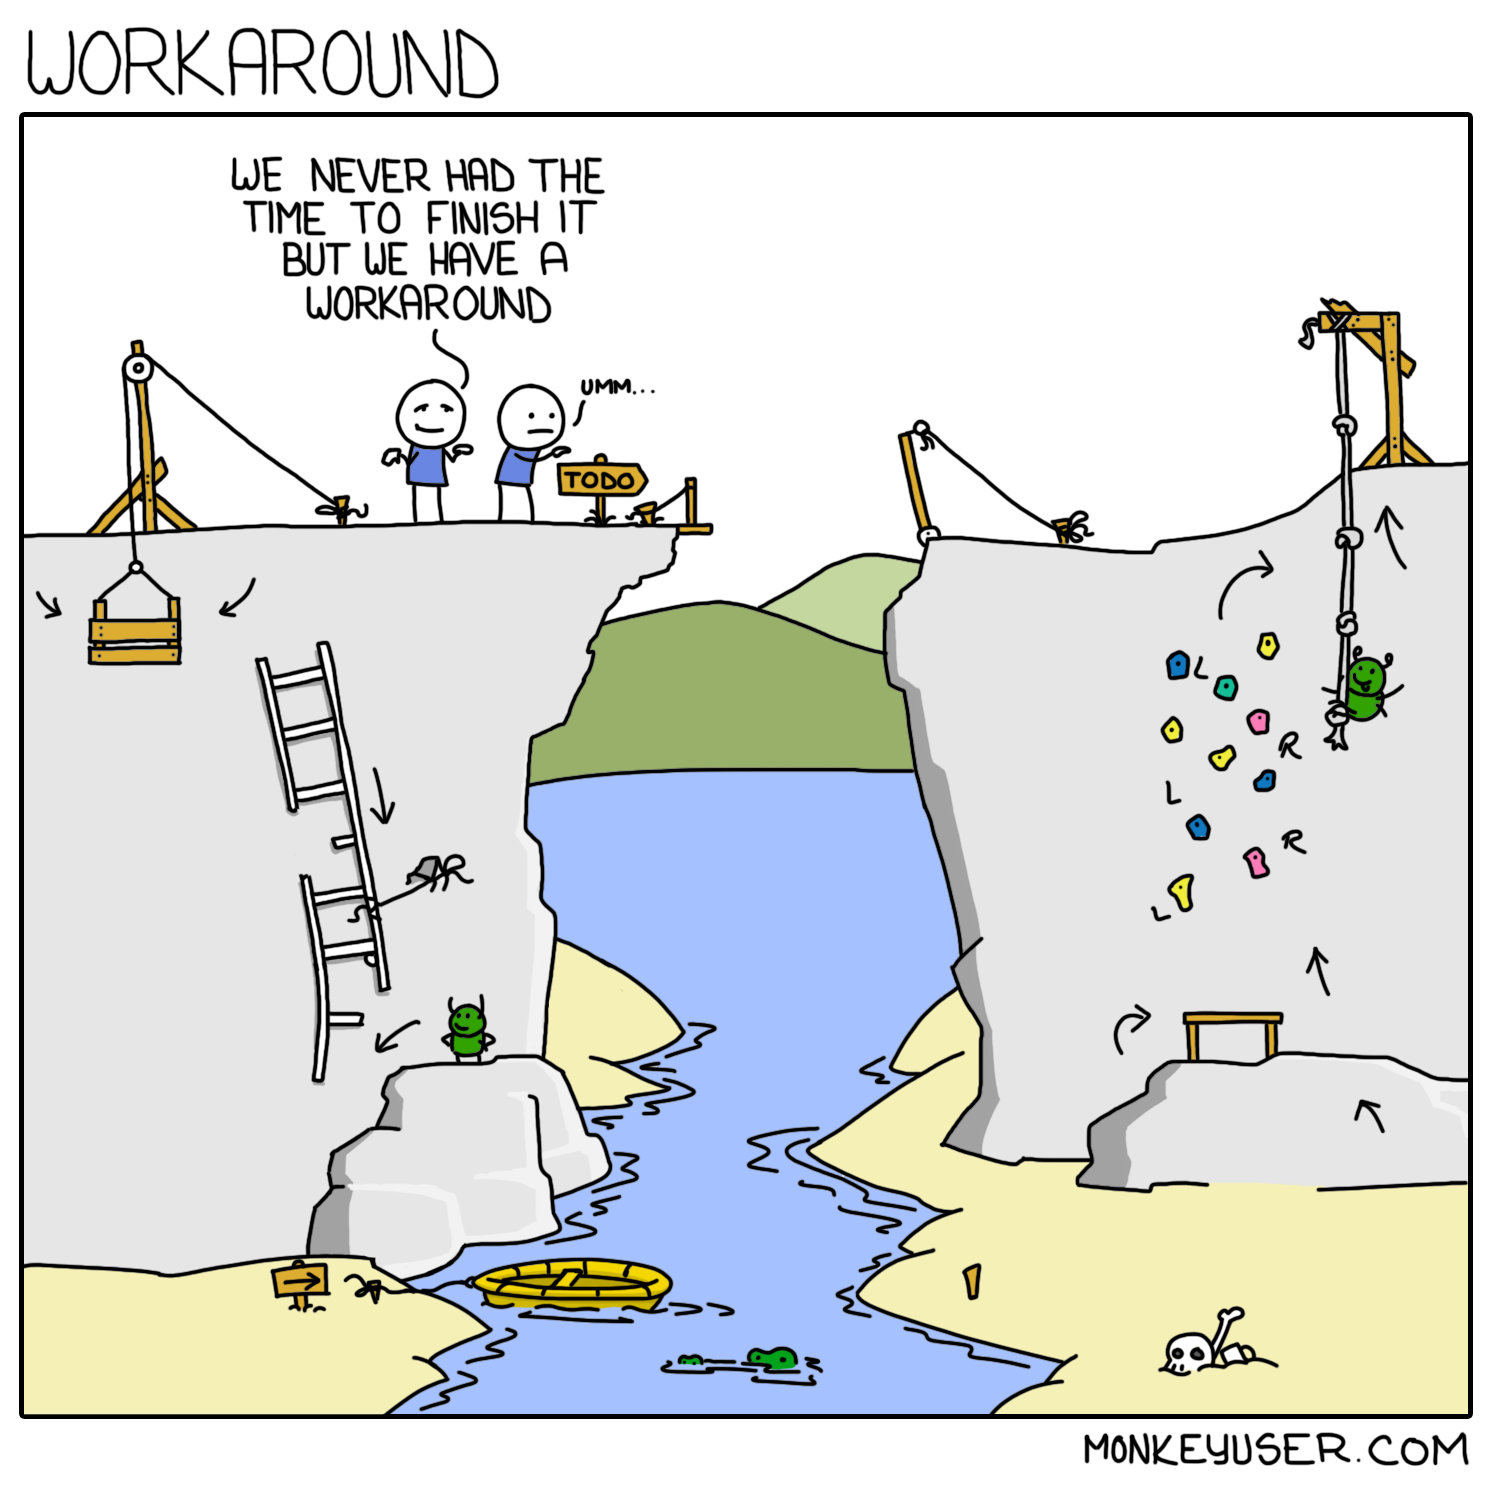
\includegraphics[scale=0.07]{Todo}};
                    \path[thin, to] ($(TD.south)!0.5!(TD.south east)$) edge[out=270, in=0] (todoEnd);
                \end{tikzpicture}
            \end{onlyenv}
        \end{onlyenv}
        \begin{onlyenv}<1-3>
            \vspace{-1mm}
            \begin{varblock}{block example}[0.98\textwidth]{Informative comment}
                \begin{lstlisting}[style=MyCpp]
                    // Format matched:     hh:mm:ss dd Month yyyy
                    std::regex timePattern("(\\d{2}:){2}\\d{2}, \\d{2} \\S+ \\d{4}");
                \end{lstlisting}
            \end{varblock}
            \begin{varblock}{block example}[0.77\textwidth]{Explanation of intent}<uncover@2->
                \begin{lstlisting}[style=MyCpp]
                    // Checking the residuum possibly not every
                    // iteration allows for speed up on GPUs
                    if(iterationNumber % CG_CHECK_RESIDUUM_EVERY == 0)
                \end{lstlisting}
            \end{varblock}
            \begin{varblock}{block example}[0.77\textwidth]{Clarification when using cryptic external API}<uncover@3>
                \begin{lstlisting}[style=MyCpp]
                    // Check if root was found up to desired precision
                    if(gsl_fcmp(functionValue, 0.0, epsilon) == 0)
                \end{lstlisting}
            \end{varblock}
        \end{onlyenv}
        \begin{varblock}{block example}[0.99\textwidth]{Amplification}<only@4>
            \begin{lstlisting}[style=MyCpp]
                // See https://stackoverflow.com/a/1736040 for more information.
                template<typename T>
                std::string getDefaultForHelper(const T& number)
            \end{lstlisting}
        \end{varblock}
        \vspace{-1mm}
        \begin{varblock}{block example}[0.99\textwidth]{}<only@4>
            \begin{lstlisting}[style=MyCpp]
                // Removing trailing spaces is crucial since any would break the
                // following algorithm. It might leave the string unchanged, but
                // the absence of trailing spaces is at the moment not guaranteed!
                boost::trim_right(keyToDecipher);
            \end{lstlisting}
        \end{varblock}
        \begin{onlyenv}<5>
            \begin{varblock}{block example}[0.98\textwidth]{TODO comments}
                \begin{lstlisting}[style=MyCpp]
                    // TODO: The following two classes should be merged into one!
                \end{lstlisting}
            \end{varblock}
            \vspace{-2mm}
            \begin{varblock}{block example}[0.7\textwidth]{Legal comments}
                \begin{lstlisting}[style=MyCpp]
                    /*******************************************
                     *  Copyright (c) 2018 Alessandro Sciarra  *
                     *                                         *
                     *  This file is part of BaHaMAS.          *
                     *******************************************/
                \end{lstlisting}
            \end{varblock}
        \end{onlyenv}
        \vspace{-5mm}
        \begin{varblock}{block alerted}[0.96\textwidth]{Automatic documentation comments}<6>
            If you are writing a public API, then you should certainly provide a good documentation.
            But be aware that documentation comments can be as misleading, misplaced and lying as any other comment.
        \end{varblock}
    \end{overlayarea}
\end{frame}
%~~~~~~~~~~~~~~~~~~~~~~~~~~~~~~~~~~~~~~~~~~~~%
\begin{frame}[fragile]{Bad comments}
    \begin{overlayarea}{\textwidth}{\textheight}
        \begin{onlyenv}<1>
            \vspace{-3mm}
            \begin{varblock}{block example}[0.94\textwidth]{Several bad habits in one example}<only@1>
                \begin{lstlisting}[style=MyCpp]
                    /**
                    * @param longTitle The complete title of the CD
                    * @param longAuthor The complete author of the CD
                    * @param nTracks The number of tracks of the CD
                    * @param durationInMinutes The duration of the CD in minutes
                    */
                    void Jukebox::addCD(std::string longTitle,
                                        std::string longAuthor,
                                        /*int nTracks,*/ int durationInMinutes)
                    {
                        // Create new CD to be later added to the list
                        CD cd;
                        cd.title    = longTitle;
                        cd.author   = longAuthor;
                        //cd.tracks   = nTracks;
                        cd.duration = durationInMinutes;
                        if(cd.duration<60) // Added by James
                           throw std::invalid_argument();
                        cdList.push_back(cd);
                    } // addCD method
                \end{lstlisting}
            \end{varblock}
        \end{onlyenv}
        \begin{onlyenv}<2>
            \begin{varblock}{block example}[0.7\textwidth]{The same code cleaned up}
                \begin{lstlisting}[style=MyCpp]
                    void Jukebox::addCD(std::string longTitle,
                                        std::string longAuthor,
                                        int durationInMinutes)
                    {
                        CD cd;
                        cd.title    = longTitle;
                        cd.author   = longAuthor;
                        cd.duration = durationInMinutes;
                        if(cd.duration<60)
                            throw std::invalid_argument();
                        cdList.push_back(cd);
                    }
                \end{lstlisting}
            \end{varblock}
            \vspace{-2mm}
            \begin{varblock}{block example}[0.7\textwidth]{}
                The code becomes smaller and it reads well!\\
                Why should you add a comment here?!
            \end{varblock}
        \end{onlyenv}
        \begin{onlyenv}<3>
            \vspace{3mm}
            \begin{itemize}
                \item Redundant comments               \hfill\makebox[55mm][l]{\PP{$\;\to\;$}\alert{Avoid}}
                \item Noise comments                   \hfill\makebox[55mm][l]{\PP{$\;\to\;$}\alert{Avoid}}
                \item Misleading comments              \hfill\makebox[55mm][l]{\PP{$\;\to\;$}\alert{Avoid}}
                \item Comments instead of a good name  \hfill\makebox[55mm][l]{\PP{$\;\to\;$}\PS{Use good name}}
                \item Closing brace comments           \hfill\makebox[55mm][l]{\PP{$\;\to\;$}\PB{Rarely}}
                \item Attribution comments             \hfill\makebox[55mm][l]{\PP{$\;\to\;$}\alert{Delete, use version control}}
                \item Commented-out code               \hfill\makebox[55mm][l]{\PP{$\;\to\;$}\alert{Delete, use version control}}
                \item Unclear, cryptic comments        \hfill\makebox[55mm][l]{\PP{$\;\to\;$}\alert{Remove or clarify}}
            \end{itemize}
            \begin{center}
                \large
                Have \textbf{\tikzmark{GR1}good reasons\tikzmark{GR2}} before adding a comment!
            \end{center}
            \begin{tikzpicture}[remember picture, overlay]
                \node[anchor=north, font=\footnotesize, text=ALERT] at ($(GR1)!0.5!(GR2)-(0,2mm)$) {Are they?};
            \end{tikzpicture}
        \end{onlyenv}
    \end{overlayarea}
\end{frame}
%~~~~~~~~~~~~~~~~~~~~~~~~~~~~~~~~~~~~~~~~~~~~%
\begin{frame}{Formatting}{Yes, formatting is important!}
    \begin{onlyenv}<1-4>
        \begin{varblock}{alert}[0.6\textwidth]{The 3 most important rules:}
            \begin{enumerate}[<+(1)->]
                \item Stay coherent with what you find
                \item Stay coherent with what you find
                \item Stay coherent with what you find
            \end{enumerate}
        \end{varblock}
        \vspace{-2mm}
        \begin{varblock}{alert}[0.7\textwidth]{}<uncover@4>
            \textbf{This starts with but it is not limited to formatting!}
        \end{varblock}
        \vspace{-2mm}
        \begin{varblock}{alert}[0.85\textwidth]{}<uncover@4>
            Especially important when working on an existing codebase!
        \end{varblock}
    \end{onlyenv}
    \begin{onlyenv}<5>
        \vspace{-2mm}
        \begin{itemize}
            \item How big should be a file? \\ $\to\;$ Try to stay \PP{below few hundreds}, the reader will be grateful!
            \item Give some vertical breath to your code
            \item Care about length of lines (\PP{80} to \alert{140} characters) \\
            $\to\;$ Crucial if the code is readable from browser (e.g. \PP{GitHub})
            \item Consider horizontal alignment and spacing (e.g. \PP{around operators})
            \item Be coherent (e.g. \PP{braces})
        \end{itemize}
        \vspace{-1mm}
        \begin{varblock}{alert}[0.9\textwidth]{How to work when different people write in the same code base?}
            Agree on a style and \alert{use a tool} (e.g.\ clang-format) to enforce it
        \end{varblock}
    \end{onlyenv}
\end{frame}
%===================================================================================================%


%===================================================================================================%
\subsection{Documentation}
%~~~~~~~~~~~~~~~~~~~~~~~~~~~~~~~~~~~~~~~~~~~~%
\begin{frame}{Some tension}
    \begin{onlyenv}<2>
        \begin{columns}
            \hfill
            \begin{column}{0.45\textwidth}
                
\includegraphics[width=\textwidth]{Documentation-self-explanatory}
            \end{column}
            \begin{column}{0.45\textwidth}
                
\includegraphics[width=\textwidth]{Documentation-not-read}
            \end{column}
            \hfill
        \end{columns}
    \end{onlyenv}
    \begin{onlyenv}<3>
        \begin{center}
            
\includegraphics[width=0.7\textwidth]{Documentation-up-to-date}
        \end{center}
    \end{onlyenv}
\end{frame}
%~~~~~~~~~~~~~~~~~~~~~~~~~~~~~~~~~~~~~~~~~~~~%
\begin{frame}{Never forget it!}
    \begin{onlyenv}<1-2>
        \begin{varblock*}{quote}[0.7\textwidth]{Software testing}[Riona MacNamara, Google]
             A professionalized discipline integrated into the software development process.
        \end{varblock*}
        \vspace{3mm}
        \begin{varblock}{alert}[0.7\textwidth]{Software documentation}<uncover@2>
             A professionalized discipline integrated into the software development process
        \end{varblock}
    \end{onlyenv}
    \begin{onlyenv}<3-4>
        \begin{varblock*}{example}[0.85\textwidth]{It is about culture and mind setup}
            \begin{enumerate}
                \item Writing documentation belongs to code development!
                \item Code changes can invalidate documentation!
                \item Good testing code documents your codebase
            \end{enumerate}
        \end{varblock*}
        \vspace{3mm}
        \begin{varblock}{alert}[\textwidth]{Writing documentation is boring and people do not read it!}<uncover@4>
            That's why \textbf{you need to find the best compromise for your project}.\\[1mm]
            What's the best approach?
            What's your documentation for?\\
            Is that detail needed to be documented?
        \end{varblock}
    \end{onlyenv}
\end{frame}
%~~~~~~~~~~~~~~~~~~~~~~~~~~~~~~~~~~~~~~~~~~~~%
\begin{frame}{Choose your tool carefully}
    \def\SphinxWeb{https://www.sphinx-doc.org/en/master/}
    \def\DoxygenWeb{https://www.doxygen.nl}
    \def\MkdocsWeb{https://www.mkdocs.org}
    \def\DocsifyWeb{https://docsify.js.org/}
    \begin{center}
        \begin{tikzpicture}[node distance=5mm]
            \foreach \l [count=\n from 1, count=\nm from 0] in {Sphinx, Doxygen, Mkdocs, Docsify}{
                \ifnum\n=1
                    \node[draw, label={[font=\small]270:{\URL*{\csname\l Web\endcsname}{\l}}}] (L\n) at (0,0)
                        {\includegraphics[height=12mm]{Logo-\l}};
                \else
                    \node[draw, label={[font=\small]270:{\URL*{\csname\l Web\endcsname}{\l}}}, right = of L\nm] (L\n)
                        {\includegraphics[height=12mm]{Logo-\l}};
                \fi
            }
            \node[draw, right=of L4] {...};
        \end{tikzpicture}
    \end{center}
    \begin{varblock}{example}[0.75\textwidth]{The list of tools is longer than you might think}
        There are even \URL*{https://dev.to/doctave/how-google-twitter-and-spotify-built-a-culture-of-documentation-3e0m}{lists of tools} available!
    \end{varblock}
\end{frame}
%~~~~~~~~~~~~~~~~~~~~~~~~~~~~~~~~~~~~~~~~~~~~%
\begin{frame}{It is all about the mind setup!}
    \begin{varblock}{quote}[0.85\textwidth]{A software engineer}
         {}[...] many overestimate the cost of maintaining documentation.
         If you have a system in place, incremental improvements to docs don't have to be a huge burden that suck time away from other engineering tasks.
    \end{varblock}
    \begin{varblock}{quote}[0.85\textwidth]{Another software engineer}
         And underestimate the damage that inaccurate docs have on users' opinions.
         \alert{Once a user discovers inaccurate content, they are leery of trusting anything else you say.}
    \end{varblock}
\end{frame}
%===================================================================================================%


%===================================================================================================%
\subsection{Functions and classes}
%~~~~~~~~~~~~~~~~~~~~~~~~~~~~~~~~~~~~~~~~~~~~%
\begin{frame}[fragile]{Common general aspects}
    \vspace{-1mm}
    \begin{overlayarea}{\textwidth}{\textheight}
        \begin{varblock}{block alerted}[0.5\textwidth]{SMALL}
            Do \alert{one} thing. Do it \alert{well}. Do it \alert{only}!
        \end{varblock}
        \begin{itemize}[<only@1-3,5>]
            \item Functions and classes interfaces should stay small (see next slide)
            \item \tc<2>{PP}{Classes should fulfil the single responsibility principle}
            \item \tc<3>{PP}{One level of abstraction per function}
        \end{itemize}
        \begin{onlyenv}<3>
            \begin{center}
                \begin{minipage}{0.65\textwidth}
                    \begin{enumerate}
                        \item Let's start with an example of bad code
                        \item and then have a look to how it should be
                    \end{enumerate}
                \end{minipage}
            \end{center}
        \end{onlyenv}
        \vspace{-2mm}
        \begin{varblock}{block example}[0.51\textwidth]{Single-responsibility class}<only@2>
            \begin{lstlisting}[style=MyCpp]
                class Version {
                  public:
                    int majorNumber();
                    int minorNumber();
                    int buildNumber();
                  private:
                    // [...]
                };
            \end{lstlisting}
        \end{varblock}
        \begin{varblock}{block example}[0.85\textwidth]{Impolite, rude code $\to$ up and down to understand it!}<only@4>
            \begin{lstlisting}[style=MyCpp]
                void Machine::MakeCoffee(const Coffee& typeOfCoffee){
                    auto neededT = temperature(typeOfCoffee);
                    if(neededT < 100)
                        warmUp(neededT);
                    while(grinder_ != nullptr)
                        prepareGrinder();
                    grind(calculateGrams(typeOfCoffee));
                    auto neededP = pressure(typeOfCoffee);
                    prepareToBrew(neededT, neededP);
                    if(status_ == READY_TO_BREW)
                        brew(typeOfCoffee);
                    else
                        throw std::runtime_error("Unable to brew!");
                }
            \end{lstlisting}
        \end{varblock}
        \begin{varblock}{block example}[0.85\textwidth]{Single-level-of-abstraction function}<only@5>
            \begin{lstlisting}[style=MyCpp]
                void Machine::MakeCoffee(const Coffee& typeOfCoffee){
                    WarmUpMachineIfNeeded(typeOfCoffee);
                    GrindCoffee(typeOfCoffee);
                    SetPressureAndTemperature(typeOfCoffee);
                    BrewCoffee(typeOfCoffee);
                }
            \end{lstlisting}
        \end{varblock}
    \end{overlayarea}
\end{frame}
%~~~~~~~~~~~~~~~~~~~~~~~~~~~~~~~~~~~~~~~~~~~~%
\begin{frame}[fragile]{More about this one-thing idea}
    \begin{overlayarea}{\textwidth}{0.85\textheight}
        \begin{varblock}{quote}[0.75\textwidth]{How big should a function be?}[Robert C. Martin]<only@1,3>
            \uncover<3>{
                A function should do one thing.
                But what's one thing?\\
                \alert{A function does one thing, if you cannot meaningfully extract another function from it.}
            }
        \end{varblock}
        \begin{varblock}{block example}[0.85\textwidth]{Back to our example}<only@2>
            \begin{lstlisting}[style=MyCpp]
                void Machine::MakeCoffee(const Coffee& typeOfCoffee){
                    // 1. WarmUpMachineIfNeeded
                    auto neededT = temperature(typeOfCoffee);
                    if(neededT < 100)
                        warmUp(neededT);
                    // 2. GrindCoffee
                    while(grinder_ != nullptr)
                        prepareGrinder();
                    grind(calculateGrams(typeOfCoffee));
                    // 3. SetPressureAndTemperature, needs T again
                    auto neededP = pressure(typeOfCoffee);
                    prepareToBrew(neededT, neededP);
                    // 4. BrewCoffee
                    if(status_ == READY_TO_BREW)
                        brew(typeOfCoffee);
                    else
                        throw std::runtime_error("Unable to brew!");
                }
            \end{lstlisting}
        \end{varblock}
        \begin{varblock}{block example}[0.85\textwidth]{Result after extraction}<only@3>
            \begin{lstlisting}[style=MyCpp]
                void Machine::MakeCoffee(const Coffee& typeOfCoffee){
                    WarmUpMachineIfNeeded(typeOfCoffee);
                    GrindCoffee(typeOfCoffee);
                    SetPressureAndTemperature(typeOfCoffee);
                    BrewCoffee(typeOfCoffee);
                }
            \end{lstlisting}
        \end{varblock}
    \end{overlayarea}
\end{frame}
%~~~~~~~~~~~~~~~~~~~~~~~~~~~~~~~~~~~~~~~~~~~~%
\begin{frame}[fragile]{Limit the number of arguments}{Make useful abstractions whenever it helps}
    \begin{varblock}{block example}[\textwidth]{When you call the function, which argument is what?}
        \begin{lstlisting}[style=MyCpp]
            double Distance(double, double, double, double);
            double Distance(double, double, double, double, double, double);
        \end{lstlisting}
    \end{varblock}
    \begin{tikzpicture}
        \path coordinate (A) at (0,0) coordinate (B) at (3,1);
        \fill[PB] (A) circle[radius=1mm]; \fill[PB] (B) circle[radius=1mm];
        \draw[<->, >=stealth, shorten <= 4pt, shorten >= 4pt] (A) -- (B);
        \node[left = 2mm of A] {$A$};
        \node[right = 2mm of B] {$B$};
    \end{tikzpicture}
    \vspace{-1mm}
    \begin{varblock}{block example}[0.72\textwidth]{Isn't this much better?}<uncover@2>
        \begin{lstlisting}[style=MyCpp]
            struct Point2D {           struct Point3D {
                double x, y;               double x, y, z;
            };                         };

            double Distance(std::pair<Point2D, Point2D>);
            double Distance(std::pair<Point3D, Point3D>);
        \end{lstlisting}
    \end{varblock}
    \begin{tikzpicture}[remember picture, overlay]
        \draw[visible on=<2>, thick] ($(current page.center)-(0.2,1.7)$) -- ++(0,-1);
    \end{tikzpicture}
\end{frame}
%===================================================================================================%


%===================================================================================================%
\subsection{IOSP}
%~~~~~~~~~~~~~~~~~~~~~~~~~~~~~~~~~~~~~~~~~~~~%
\begin{frame}[fragile]{\PQ{I}ntegration \PQ{O}peration \PQ{S}egregation \PQ{P}rinciple}
    \begin{overlayarea}{\textwidth}{0.85\textheight}
        \vspace{-3mm}
        \begin{varblock}{block alerted}[\textwidth]{Clear separation of:}
            \begin{description}
                \item[Operation:]   A function which contains exclusively logic, meaning transformations, control structures or API invocations.
                \item[Integration:] A function which does not contain any logic but exclusively calls other functions of the code base.
            \end{description}
        \end{varblock}
        \vspace{-1mm}
        \begin{varblock}{block example}[0.75\textwidth]{Operation}<only@1>
            \begin{lstlisting}[style=MyCpp]
                bool isPrime(unsigned int number)
                {
                    if(number == 1) return false;
                    for(auto i = 2u; i <= std::sqrt(number); ++i)
                    {
                        if(number%i == 0) return false;
                    }
                    return true;
                }
            \end{lstlisting}
        \end{varblock}
        \begin{varblock}{block example}[0.62\textwidth]{Integration}<only@2>
            \begin{lstlisting}[style=MyCpp]
                int main(int argc, char *argv[])
                {
                    WelcomeUserToTheGame();
                    Minesweeper minesweeper(argc, argv);
                    minesweeper.playGame();
                    PrintGameResult();
                }
            \end{lstlisting}
        \end{varblock}
    \end{overlayarea}
\end{frame}
%===================================================================================================%
    \session{lecture}{Clean testing (II)}
    %-------------------------------%
%  Author: Alessandro Sciarra   %
%    Date: 02 Jul 2025          %
%-------------------------------%

%===================================================================================================%
\subsection{The curse of the \textbf{unit} word}
%~~~~~~~~~~~~~~~~~~~~~~~~~~~~~~~~~~~~~~~~~~~~%
\begin{frame}{What is a \textbf{unit} in unit testing?}
    \begin{overlayarea}{\textwidth}{0.38\textheight}
        \begin{onlyenv}<1>
            \begin{varblock}{quote}[0.7\textwidth]{}[Wikipedia]
                A group of related functions often called a module.
            \end{varblock}
            \begin{varblock}{quote}[0.7\textwidth]{}[Ian Cooper]
                A unit test should test a requirement, only test against the stable contract of the API.
            \end{varblock}
        \end{onlyenv}
        \begin{onlyenv}<2>
            \vspace{-4mm}
            \begin{center}
                
\includegraphics[width=0.7\textwidth]{Fragile-test-problem}
            \end{center}
        \end{onlyenv}
    \end{overlayarea}
    \begin{varblock}{alert}[0.98\textwidth]{A unit is not necessarily a class or a function}
        This is possibly one of the most misunderstood concepts in software engineering in the last decade.
        Sometimes a unit is a class or a function, but there should be a good reason for such a correspondence.
        \textbf{More often a unit should be (the public API of) a module.}
    \end{varblock}
\end{frame}
%~~~~~~~~~~~~~~~~~~~~~~~~~~~~~~~~~~~~~~~~~~~~%
\AlertFrame{
    \begin{tabular}{c}
        Wait, what's wrong\\ in testing each single class?
    \end{tabular}
}
%~~~~~~~~~~~~~~~~~~~~~~~~~~~~~~~~~~~~~~~~~~~~%
\begin{frame}{It depends}
    \vspace{-3mm}
    \begin{varblock}{quote}[0.8\textwidth]{TDD, Where Did It All Go Wrong}[Ian Cooper]
        A couple of times we were very proud of the fact that we produced some code that went to production with almost zero defects.
        [...]
        I looked at this test suite.
        One things I noticed was that \alert{we had about three times as much test code as production code}.
    \end{varblock}
    \begin{itemize}
        \item Some classes are simply implementation details\\
        \then You would like to freely change them
        \item Imagine a module with few classes working together \Remark{in your implementation, today}\\
        \then Does it make sense to mock all but one several times?
        \item If a class happens to be the API of a module, probably that's a unit
    \end{itemize}
\end{frame}
%===================================================================================================%


%===================================================================================================%
\subsection[White- and black-box testing!?]{The weaknesses of white- and black-box testing}
%~~~~~~~~~~~~~~~~~~~~~~~~~~~~~~~~~~~~~~~~~~~~%
\AlertFrame{
    \begin{tabular}{c}
        I'll test a single class next in examples,\\
        but you now know what a \textbf{unit} is!
    \end{tabular}
}
%~~~~~~~~~~~~~~~~~~~~~~~~~~~~~~~~~~~~~~~~~~~~%
\begin{frame}[fragile]{White box testing}
    \vspace{-3mm}
    \begin{overlayarea}{\textwidth}{0.7\textheight}
        \begin{itemize}
            \item You allow yourself in using all code in your tests\\
            \begin{onlyenv}<1>
                \then even private methods and members\\
                \then implementation details are used to test interface
            \end{onlyenv}
            \item<2-> In some languages (e.g.\ Python) easier than in others (e.g.\ C++)
            \item<only@5-> \PS{Something to consider to start working on legacy code!}\\
            \item<only@6> \alert{What happens when you change your implementation?}\\
            \then Compilation might break\\
            \then If not, some tests will probably fail\\
            \then You likely need to change your tests code\\
            \then For large refactoring, it might be boring/frustrating\\[3mm]
            \centerline{\Huge\emoji{thinking-face}}
        \end{itemize}
        \begin{columns}[T]
            \begin{column}{0.45\textwidth}
                \begin{varblock}{example}[\textwidth]{Consider this class}<only@2-3>
                    \begin{lstlisting}[style=MyCpp]
                        // File Cup.h

                        class Cup {
                            public:
                            Cup();
                            bool IsEmpty();
                            bool Drink();
                            bool Fill();
                            private:
                            bool isEmpty_ = true;
                        };
                    \end{lstlisting}
                \end{varblock}
                \begin{varblock}{example}[\textwidth]{Consider this class}<only@4>
                    \begin{lstlisting}[style=MyCpp]
                        // File Cup.h

                        class Cup {
                            public:
                            Cup();
                            bool IsEmpty();
                            bool Drink();
                            bool Fill();
                            private:
                            friend struct CupTester;
                            bool isEmpty_ = true;
                        };
                    \end{lstlisting}
                \end{varblock}
            \end{column}
            \begin{column}{0.48\textwidth}
                \begin{varblock}{example}[\textwidth]{Test file}<only@2>
                    \begin{lstlisting}[style=MyCpp]
                        #include |+"vir/test.h"+|
                        #include |+"Cup.h"+|


                        TEST(|=Cup::Cup=|) {
                            Cup cup{};
                            VERIFY(cup.isEmpty_);
                        }
                        TEST(|=Cup::IsEmpty=|) { /*...*/ }
                        TEST(|=Cup::Fill=|)    { /*...*/ }
                        TEST(|=Cup::Drink=|)   { /*...*/ }
                    \end{lstlisting}
                \end{varblock}
                \begin{varblock}{example}[\textwidth]{Test file}<only@3>
                    \begin{lstlisting}[style=MyCpp]
                        #include |+"vir/test.h"+|
                        #include |+"Cup.h"+|
                        #define private public // UB!!!

                        TEST(|=Cup::Cup=|) {
                            Cup cup{};
                            VERIFY(cup.isEmpty_);
                        }
                        TEST(|=Cup::IsEmpty=|) { /*...*/ }
                        TEST(|=Cup::Fill=|)    { /*...*/ }
                        TEST(|=Cup::Drink=|)   { /*...*/ }
                    \end{lstlisting}
                \end{varblock}
                \begin{varblock}{example}[\textwidth]{Test file}<only@4>
                    \begin{lstlisting}[style=MyCpp]
                        #include |+"vir/test.h"+|
                        #include |+"Cup.h"+|
                        struct CupTester { /*...*/ };

                        TEST(|=Cup::Cup=|) {
                            Cup cup{};
                            CupTester tester{cup};
                            VERIFY(tester.isEmpty_);
                        }
                        TEST(|=Cup::IsEmpty=|) { /*...*/ }
                        TEST(|=Cup::Fill=|)    { /*...*/ }
                        TEST(|=Cup::Drink=|)   { /*...*/ }
                    \end{lstlisting}
                \end{varblock}
                \centering\vspace{-3mm}
                \only<2>{\alert{\scriptsize This does not compile!}}
                \only<3>{\alert{\scriptsize This relies on undefined behaviour!!!}}
            \end{column}
        \end{columns}
        \FrameRemark<2-4>{I took this example from Dave Steffen's talk at CppCon2020.}
    \end{overlayarea}
\end{frame}
%~~~~~~~~~~~~~~~~~~~~~~~~~~~~~~~~~~~~~~~~~~~~%
\begin{frame}[fragile]{Black-box testing}
    \vspace{-3mm}
    \begin{overlayarea}{\textwidth}{0.7\textheight}
        \begin{itemize}
            \item What about just testing the public interface?
        \end{itemize}
        \vspace{-3mm}
        \begin{columns}[T]
            \begin{column}{0.45\textwidth}
                \begin{varblock}{example}[\textwidth]{Consider this class}<only@1-3>
                    \begin{lstlisting}[style=MyCpp]
                        // File Cup.h

                        class Cup {
                            public:
                            Cup();
                            bool IsEmpty();
                            bool Drink();
                            bool Fill();
                            private:
                            bool isEmpty_ = true;
                        };
                    \end{lstlisting}
                \end{varblock}
                \centering%\vspace{-3mm}
                \only<1-3>{\scriptsize Source code same as before}
            \end{column}
            \begin{column}{0.48\textwidth}
                \begin{varblock}{example}[\textwidth]{Test file}<only@1>
                    \begin{lstlisting}[style=MyCpp]
                        #include |+"vir/test.h"+|
                        #include |+"Cup.h"+|

                        TEST(|=Cup::Cup=|)     { /*...*/ }
                        TEST(|=Cup::IsEmpty=|) { /*...*/ }
                        TEST(|=Cup::Fill=|)    { /*...*/ }
                        TEST(|=Cup::Drink=|)   { /*...*/ }
                    \end{lstlisting}
                \end{varblock}
                \begin{varblock}{example}[\textwidth]{Test file}<only@2>
                    \begin{lstlisting}[style=MyCpp]
                        #include |+"vir/test.h"+|
                        #include |+"Cup.h"+|

                        TEST(|=Cup::Cup=|) {
                            Cup cup{};
                            VERIFY(cup.IsEmpty());
                        }
                        TEST(|=Cup::IsEmpty=|) { /*...*/ }
                        TEST(|=Cup::Fill=|)    { /*...*/ }
                        TEST(|=Cup::Drink=|)   { /*...*/ }
                    \end{lstlisting}
                \end{varblock}
                \begin{varblock}{example}[\textwidth]{Test file}<only@3>
                    \begin{lstlisting}[style=MyCpp]
                        #include |+"vir/test.h"+|
                        #include |+"Cup.h"+|

                        TEST(|=Cup::Cup=|) {
                            Cup cup{};
                            VERIFY(cup.IsEmpty());
                        }
                        TEST(|=Cup::IsEmpty=|){
                            Cup cup{};
                            VERIFY(cup.IsEmpty());
                        }
                        TEST(|=Cup::Fill=|)    { /*...*/ }
                        TEST(|=Cup::Drink=|)   { /*...*/ }
                    \end{lstlisting}
                \end{varblock}
            \end{column}
        \end{columns}
        \begin{onlyenv}<3>
            \begin{center}
                \alert{Wait, we wrote the same code twice!}
            \end{center}
        \end{onlyenv}
        \vspace{-3mm}
        \begin{varblock}{quote}[0.8\textwidth]{The black-box conundrum}[Dave Steffen]<only@4-5>
            Fundamentally if we only test via the public interface, we have a circular-logic problem: you have to use the interface to test the interface, so at some point you have to trust something which you haven't tested.
        \end{varblock}
        \begin{varblock}{alert}[0.95\textwidth]{So, what to do then?}<only@5>
            \begin{enumerate}
                \item Ignore the problem \Remark{Be aware: Tests are not independent, one bug triggers many failures!}
                \item Declare one member function ``correct by inspection'' \Remark{and start from there}
                \item Abandon black-box testing as impractical
            \end{enumerate}
        \end{varblock}
    \end{overlayarea}
\end{frame}
%===================================================================================================%


%===================================================================================================%
\subsection{Test the behaviour, not the implementation}
%~~~~~~~~~~~~~~~~~~~~~~~~~~~~~~~~~~~~~~~~~~~~%
\begin{frame}[fragile]{Do not test methods! Test behaviour!}
    \vspace{-11mm}
    \begin{overlayarea}{\textwidth}{0.7\textheight}
        \begin{varblock}{example}[0.75\textwidth]{Back to our cup example:}<only@1>
            \begin{lstlisting}[style=MyCpp]
                #include |+"vir/test.h"+|
                #include |+"Cup.h"+|

                TEST(|=A new cup is empty=|)            { /*...*/ }
                TEST(|=An empty cup can be filled=|)    { /*...*/ }
                TEST(|=A filled cup is full=|)          { /*...*/ }
                TEST(|=Drinking empties a filled cup=|) { /*...*/ }
            \end{lstlisting}
        \end{varblock}
        \begin{varblock}{example}[0.75\textwidth]{Back to our cup example:}<only@2-3>
            \begin{lstlisting}[style=MyCpp]
                #include |+"vir/test.h"+|
                #include |+"Cup.h"+|

                TEST(|=A new cup is empty=|){
                    Cup cup{};
                    VERIFY(cup.IsEmpty());
                }
                TEST(|=An empty cup can be filled=|)    { /*...*/ }
                TEST(|=A filled cup is full=|)          { /*...*/ }
                TEST(|=Drinking empties a filled cup=|) { /*...*/ }
            \end{lstlisting}
        \end{varblock}
        \only<1-3>{\vspace{3mm}}
        \begin{itemize}
            \item<only@1> Test names describe the unit specifications
            \item<only@1> Suddenly, we are completely independent from implementation details
            \item<only@1> OK, so how does test code look like?
            \item<only@3> \alert{Wait!! This is exactly the same code that wasn't OK few minutes ago!?}\\
            \then How is it that changing the name makes it fine?\\
            \then How should this solve the black-box conundrum?
        \end{itemize}
        \begin{onlyenv}<4->
            \begin{varblock}{example}[0.6\textwidth]{The bottom line}
                We are now testing consistency of interface, not correctness of implementation!
            \end{varblock}
            \begin{varblock}{alert}[0.6\textwidth]{Let's say it once more:}<5->
                \textbf{We are now testing consistency of interface, not correctness of implementation!}
            \end{varblock}
            \begin{varblock}{}[0.9\textwidth]{It is not a philosophical statement!}<6>
                \PB{A bug that cannot be observed under any conditions is not a bug!}
            \end{varblock}
        \end{onlyenv}
    \end{overlayarea}
\end{frame}
%~~~~~~~~~~~~~~~~~~~~~~~~~~~~~~~~~~~~~~~~~~~~%
\begin{frame}[fragile]{\uncover<2>{As testing behaviour passes, the code is correct!}}
    \begin{varblock}{example}[0.9\textwidth]{Is this code correct or wrong?}
        \begin{lstlisting}[style=MyCpp]
            // File Cup.h

            class Cup {
                public:
                Cup()          { isEmpty_ = false; }
                bool IsEmpty() { return !isEmpty_; }
                bool Drink()   { /*...*/ }
                bool Fill()    { /*...*/ }
                private:
                bool isEmpty_ = false;
            };
        \end{lstlisting}
    \end{varblock}
    \vspace{-2mm}
    \begin{varblock}{example}[0.9\textwidth]{}<2>
        \begin{lstlisting}[style=MyCpp]
            #include |+"vir/test.h"+|
            #include |+"Cup.h"+|
            TEST(|=A new cup is empty=|)            { /*...*/ }
            TEST(|=An empty cup can be filled=|)    { /*...*/ }
            TEST(|=A filled cup is full=|)          { /*...*/ }
            TEST(|=Drinking empties a filled cup=|) { /*...*/ }
        \end{lstlisting}
    \end{varblock}
\end{frame}
%===================================================================================================%

    \session{exercise}{The time has come}
    %-------------------------------%
%  Author: Alessandro Sciarra   %
%    Date: 02 Jul 2025          %
%-------------------------------%

%~~~~~~~~~~~~~~~~~~~~~~~~~~~~~~~~~~~~~~~~~~~~%
\begin{frame}{A new begin}{You have 90 minutes}
    \begin{enumerate}
        \setcounter{enumi}{-1}
        \item You won't work on your code! $\;\to\;$ \Emoji[\huge]{recycling-symbol}
        \item Improve names!\\
              \then Your IDE can probably rename symbols
        \item Check comments $\;\to\;$ Remove or add (is there a good reason?)
        \item Is there documentation? If not, how would you add some?\\
              \then Any thoughts about that?
        \item \PS{Add some tests for one or more functions}
        \item Apply IOSP to such functions\\
              \then How do you pass around arguments?
        \item \alert{Stage, commit and push your work!}
    \end{enumerate}
    \begin{tikzpicture}[remember picture, overlay]
        \node[anchor=south east] at ($(current page.south east)+(-0.5,1)$) {
\includegraphics[width=0.25\textwidth]{Feeling-good}};
        \node[anchor=north east] at ($(current page.north east)-(0.5,0.3)$) {
\includegraphics[width=0.20\textwidth]{Psychopath}};
    \end{tikzpicture}
\end{frame}
%~~~~~~~~~~~~~~~~~~~~~~~~~~~~~~~~~~~~~~~~~~~~%

    \session{lecture}{Clean testing (III)}
    %-------------------------------%
%  Author: Alessandro Sciarra   %
%    Date: 02 Jul 2025          %
%-------------------------------%

%===================================================================================================%
\subsection{Tests goals -- properties -- good principles}
%~~~~~~~~~~~~~~~~~~~~~~~~~~~~~~~~~~~~~~~~~~~~%
\begin{frame}{General idea and overview}
    \begin{overlayarea}{\textwidth}{0.7\textheight}
        \begin{center}
            \large
            \only<1-2>{There is slightly different advice around, pick your favourite:}
            \only<3->{There is one not-negotiable \textbf{requirement of tests}, though:}
        \end{center}
        \begin{varblock}{example}[0.8\textwidth]{Write F.I.R.S.T tests first}<only@1>
            \begin{description}[Self-validating:]
                \item[\PQ{F}ast:] To be run frequently
                \item[\PQ{I}ndependent:] To make failures meaningful
                \item[\PQ{R}epeatable:] To be run everywhere with same outcome
                \item[\PQ{S}elf-validating:] To be automatised
                \item[\PQ{T}imely:] To make production code testable
            \end{description}
        \end{varblock}
        \begin{varblock}{example}[\textwidth]{Google's perspective}<only@2>
            \begin{description}[Self-validating:]
                \item[Readable:] Tests are correct by inspection
                \item[Correct:] Do not rely on known bugs and test real scenarios
                \item[Complete:] Test most edge cases
                \item[Documenting:] Demonstration of how the API works
                \item[Resilient:] Repeatable, independent, hard to break, hermetic, etc.
            \end{description}
        \end{varblock}
        \begin{tikzpicture}[overlay, remember picture]
            \node[starburst, starburst points=21, starburst point height=15mm,
            minimum width=10cm, minimum height=6cm, Shape={red}{yellow!50}{red},
            line width=1.5pt, font=\Huge\bfseries, visible on=<4>]
            at ($(current page.center)-(0,1)$) {Existence};
        \end{tikzpicture}
    \end{overlayarea}
\end{frame}
%~~~~~~~~~~~~~~~~~~~~~~~~~~~~~~~~~~~~~~~~~~~~%
\begin{frame}[fragile]{Having tests is not enough, you must trust them!}{Few words about tests correctness}
    \begin{overlayarea}{\textwidth}{0.7\textheight}
        \begin{itemize}
            \item Never rely on known bugs
            \item<only@4-> Never mock the code that you are testing
        \end{itemize}
        \begin{varblock}{alert}[0.6\textwidth]{Having tests passing is simple...}<only@1-2>
            \begin{uncoverenv}<2->
                \begin{lstlisting}[style=MyCpp]
                    int cube(int x) {
                        //TODO: To be implemented
                        return 0;
                    }

                    TEST(cube_test) {
                        VERIFY(0 == cube(2));
                        VERIFY(0 == cube(3));
                        VERIFY(0 == cube(42));
                    }
                \end{lstlisting}
            \end{uncoverenv}
        \end{varblock}
        \begin{varblock}{example}[0.6\textwidth]{...better to have them failing!}<only@3>
            \begin{lstlisting}[style=MyCpp]
                int cube(int x) {
                    //TODO: To be implemented
                    return 0;
                }

                TEST(cube_test) {
                    VERIFY(8 == cube(2));
                    VERIFY(27 == cube(3));
                    VERIFY(74088 == cube(42));
                }
            \end{lstlisting}
        \end{varblock}
        \begin{varblock}{alert}[0.8\textwidth]{This is probably useless}<only@4>
            \begin{lstlisting}[style=MyCpp]
                class MockCoffeeMachine : public CoffeeMachine {
                    //For simplicity we assume always in temperature
                    double warmUp() override {
                        return constants::brewingT;
                    }
                }

                BOOST_AUTO_TEST_CASE(warmUp_test) {
                    MockCoffeeMachine machine{};
                    BOOST_REQUIRE_CLOSE(machine.warmUp(),
                    constants::brewingT, 0.1);
                }
            \end{lstlisting}
        \end{varblock}
        \vspace{3mm}
        \begin{varblock}{}[0.85\textwidth]{Think of a clear reaction procedure in your team}<only@5->
            What should happen in your project when a test fails?\\
            ...and when a bug that was not caught by tests is found?\\
            $\downarrow$\\
            \PB{Never miss any chance to improve your tests!}
        \end{varblock}
    \end{overlayarea}
\end{frame}
%~~~~~~~~~~~~~~~~~~~~~~~~~~~~~~~~~~~~~~~~~~~~%
\begin{frame}{Tests readability}
    \begin{center}
        \begin{tikzpicture}[every node/.style={inner sep=0mm, text=BGLIGHT}]
            \node (fig) {
\includegraphics[width=0.75\textwidth]{Balance}};
            \begin{DrawOnNode}{fig}
                \node[anchor=east] at (0.41,0.78) {
                    \begin{tabular}{c}
                        Avoid boilerplate\\
                        \footnotesize E.g. use functions for setup\\
                    \end{tabular}
                };
                \node[anchor=west] at (0.51,0.78) {
                    \begin{tabular}{c}
                        Give enough context\\
                        \footnotesize E.g. Not a single function for setup\\
                    \end{tabular}
                };
            \end{DrawOnNode}
        \end{tikzpicture}
    \end{center}
    \begin{varblock}{}[0.85\textwidth]{}
        \Large Remember: \PB{Tests are correct by inspection!}
    \end{varblock}
\end{frame}
%~~~~~~~~~~~~~~~~~~~~~~~~~~~~~~~~~~~~~~~~~~~~%
\begin{frame}[fragile]{Tests completeness: What should I test and how?}
    \begin{onlyenv}<1>
        \begin{itemize}
            \item Values  \\ \centerline{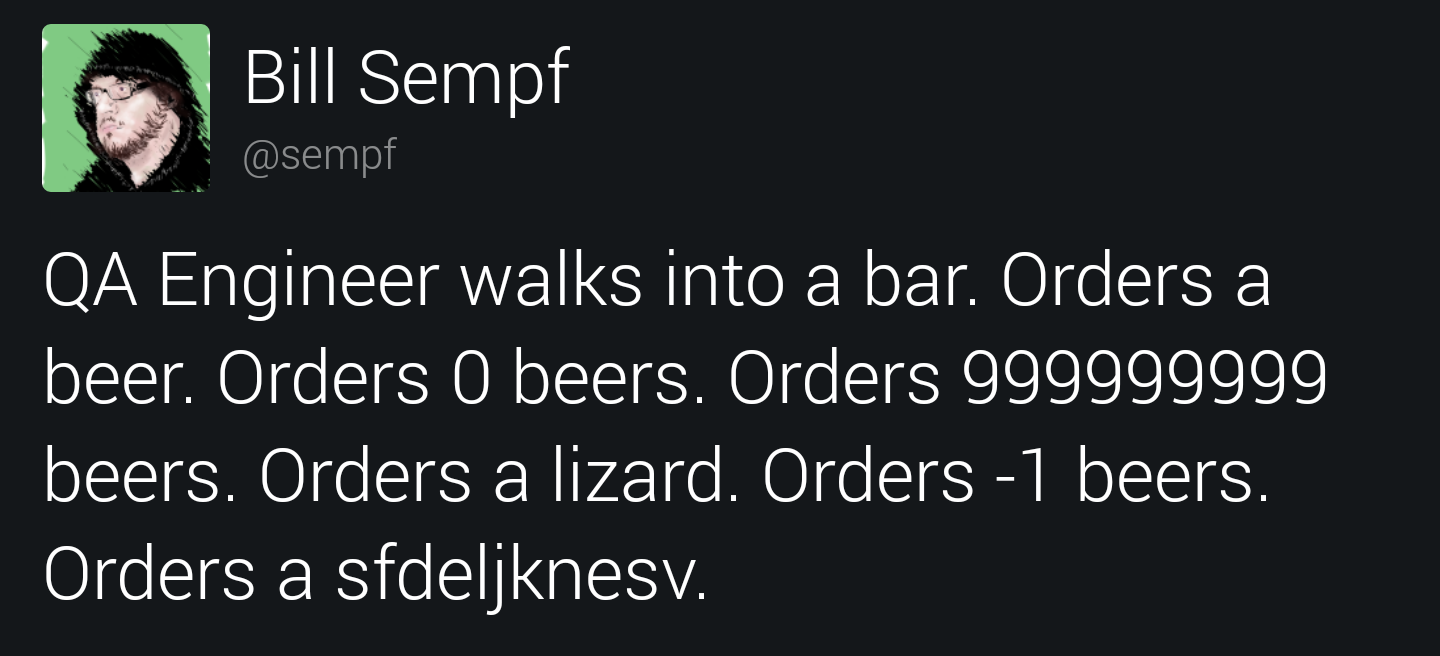
\includegraphics[scale=0.1]{Testing-value}}
            \item Actions \\ \centerline{
\includegraphics[scale=0.12, clip, trim=0 4cm 0 4cm]{Testing-action}}
        \end{itemize}
        \vspace{3mm}
        \hfill\ldots{}and anything that makes sense!
    \end{onlyenv}
    \begin{varblock}{example}[0.98\textwidth]{A very nice example from Titus Winter}<only@2->
        \begin{overlayarea}{\textwidth}{0.55\textheight}
            \begin{uncoverenv}<3->
                \begin{lstlisting}[style=MyCpp]
                    int Factorial(int n) {
                        if (n == 1) return 1;
                        if (n == 5) return 120;
                        return -1; // TODO(goofus): figure this out.
                    }
                \end{lstlisting}
            \end{uncoverenv}
            \begin{onlyenv}<2-3>
                \begin{lstlisting}[style=MyCpp]
                    TEST(FactorialTest, BasicTests) {
                        EXPECT_EQ(1, Factorial(1));
                        EXPECT_EQ(120, Factorial(5));
                    }
                \end{lstlisting}
            \end{onlyenv}
            \begin{onlyenv}<4>
                \begin{lstlisting}[style=MyCpp]
                    TEST(FactorialTest, BasicTests) {
                        EXPECT_EQ(1, Factorial(1));
                        EXPECT_EQ(120, Factorial(5));
                        EXPECT_EQ(1, Factorial(0));
                        EXPECT_EQ(479001600, Factorial(12));
                        EXPECT_EQ(std::numeric_limits<int>::max() , Factorial(13));
                        EXPECT_EQ(1, Factorial(0));
                        EXPECT_EQ(std::numeric_limits<int>::max() , Factorial(-10));
                    }
                \end{lstlisting}
            \end{onlyenv}
        \end{overlayarea}
    \end{varblock}
    \begin{uncoverenv}<4>
        \begin{center}
            This will pretty much naturally emerge when doing TDD
        \end{center}
    \end{uncoverenv}
\end{frame}
%~~~~~~~~~~~~~~~~~~~~~~~~~~~~~~~~~~~~~~~~~~~~%
\begin{frame}{The hidden value of tests}{Few words about tests as API usage examples}
    \begin{overlayarea}{\textwidth}{0.68\textheight}
        \begin{center}
            \small
            Of course, a meme, do not take it (too) seriously, but...\\
            \vspace{3mm}
            \begin{uncoverenv}<2>
                
\includegraphics[width=0.7\textwidth]{Documentation-meme}\\
                \vspace{3mm}
                ...good tests should show how to use your code!
            \end{uncoverenv}
        \end{center}
        \FrameRemark<2>{In this sense, it should be avoided to use implementation details in tests (cf. white box testing downsides).}
    \end{overlayarea}
\end{frame}
%~~~~~~~~~~~~~~~~~~~~~~~~~~~~~~~~~~~~~~~~~~~~%
\begin{frame}[fragile]{Tests resilience: Google advice}
    \begin{onlyenv}<1>
        \begin{itemize}
            \setlength{\itemsep}{2mm}
            \item No flaky tests $\to$ Tests should always give the same outcome
            \item No brittle tests $\to$ One failure should not trigger many failures
            \item Tests reference values should not come from the system under test!
            \item Changing tests order should never change the outcome
            \item Tests should be as hermetic as possible $\to$ No I/O, no network, etc.
            \item No deep dependence $\to$ Avoid any implicit assumption
        \end{itemize}
        \vspace{3mm}
        \begin{varblock}{example}[0.5\textwidth]{}
            \large\bfseries\PS{Let's see some examples!}
        \end{varblock}
    \end{onlyenv}
    \begin{onlyenv}<2-3>
        \begin{varblock}{alert}[\textwidth]{A sneaky flaky test: What happens if the test-system is overloaded?}
            \begin{lstlisting}[style=MyCpp]
                TEST(UpdaterTest, RunsFast) {
                    Updater updater;
                    updater.UpdateAsync();
                    SleepFor(Seconds(.5)); // Half a second should be *plenty*.
                    EXPECT_TRUE(updater.Updated());
                }
            \end{lstlisting}
        \end{varblock}
        \begin{varblock}{alert}[\textwidth]{An infamous brittle pattern}<uncover@3>
            \begin{lstlisting}[style=MyCpp]
                TEST(Logger, LogWasCalled) {
                    StartLogCapture();
                    EXPECT_TRUE(Frobber::Start());
                    EXPECT_THAT(
                      Logs(), Contains("file.cc:421: Opened file frobber.config" )
                    );@|\tikzmark{logger}|@
                }
            \end{lstlisting}
        \end{varblock}
        \begin{tikzpicture}[remember picture, overlay]
            \draw[red, thick, double, visible on=<3>]
                ($(logger)+(3.05,0.12)$) -- ++(1.15,0)
                +(0.18,0) -- ++(0.65,0)
                +(2.4,0) -- ++(4.8,0);
        \end{tikzpicture}
    \end{onlyenv}
    \begin{onlyenv}<4-5>
        \begin{varblock}{alert}[\textwidth]{Where are the reference values coming from?}
            \begin{lstlisting}[style=MyCpp]
                BOOST_AUTO_TEST_CASE(Dirac_M)
                {
                    const hmc_float refs[4] =
                        { 2610.3804893063798, 4356.332327032359,
                          2614.2685771909237, 4364.1408252701831 };
                    test_fermionmatrix<physics::fermionmatrix::Dslash>(refs);
                }
            \end{lstlisting}
        \end{varblock}
        \begin{varblock}{alert}[\textwidth]{A non-hermetic test: What if run twice in parallel?}<uncover@5>
            \begin{lstlisting}[style=MyCpp]
                TEST(Server, StorageTest) {
                    StorageServer* server = GetStorageServerHandle();
                    auto my_val = rand();
                    server->Store("testkey", my_val);
                    EXPECT_EQ(my_val, server->Load("testkey"));
                }
            \end{lstlisting}
        \end{varblock}
    \end{onlyenv}
    \begin{onlyenv}<6>
        \vspace{-3mm}
        \begin{varblock}{alert}[\textwidth]{Deep dependence example}<only@6>
            \begin{lstlisting}[style=MyCpp]
                class File {
                    public:
                    // ...
                    virtual bool StatWithOptions(Stat_t* stat, StatOptions opts) {
                        return this->Stat(stat); // In base class ignore options
                    }
                };
                TEST(Filesystem, FSUsage) {
                    // ... and call to StatWithOptions
                    EXPECT_CALL(file, Stat(_)).Times(1);
                }  // This relies on a call to base StatWithOptions!!
            \end{lstlisting}
        \end{varblock}
        \begin{varblock}{quote}[\textwidth]{The law of implicit interfaces (AKA Hyrum's law)}[Hyrum Wright]<only@6>
            Given enough users of your public interface, soon or later someone will start implicitly relying on your implementation details (speed, memory consumption, etc.).\\[-1.2ex]~
        \end{varblock}
    \end{onlyenv}
    \begin{uncoverenv}<1-3,5->
        \FrameRemark{This list and all GoogleTest examples are taken from Titus Winters' and Hyrum Wright's talk at CppCon2015.}
    \end{uncoverenv}
\end{frame}
%~~~~~~~~~~~~~~~~~~~~~~~~~~~~~~~~~~~~~~~~~~~~%
\begin{frame}{A slide about tests precision}
    \vspace{-3mm}
    \begin{onlyenv}<1>
        \begin{center}
            
\includegraphics[width=0.7\textwidth]{Precision-meme}
        \end{center}
    \end{onlyenv}
    \begin{onlyenv}<2>
        \begin{itemize}
            \item We all know that machine precision is finite!
            \item Comparing floating point numbers has to be done carefully
            \item If you know a reference value exactly, put in the code more than the needed digits
            \PB{$\;\to\pi=3.141592653589793238462643$}
            \item Be aware of possible compiler techniques, e.g.\ FMA \Remark{fused multiply-add}\\
            \then This could make your test fail if you require too high precision
            \item Requiring too high precision makes tests brittle
            \item Requiring too low precision makes tests useless
            \item \alert{After all it is a judgement call!}
        \end{itemize}
    \end{onlyenv}
\end{frame}
%~~~~~~~~~~~~~~~~~~~~~~~~~~~~~~~~~~~~~~~~~~~~%
\begin{frame}{Few more words about reproducibility}
    \vspace{-5mm}
    \begin{varblock}{example}[0.96\textwidth]{How can I make my tests reproducible?}
        \begin{enumerate}
            \item Isolate them from non-deterministic aspects \Remark{e.g.\ network, database, random numbers}\\
            \then This is not always possible!
            \item Measure unwanted environment effect and subtract it in tests
            \item Detect if test can be run in the present environment\\
            \then If not, either fail or handle situation
            \item \alert{Handle intrinsic noise by statistics}\\
            \Then{E.g.\ if random numbers are needed, measure the failure frequency and re-run the test a number of times large enough to consider a failure as such!}
        \end{enumerate}
    \end{varblock}
\end{frame}
%~~~~~~~~~~~~~~~~~~~~~~~~~~~~~~~~~~~~~~~~~~~~%
\begin{frame}{Tests accuracy and reacting to failures}
    \begin{center}
        \begin{tikzpicture}
            \coordinate (O) at (0,0);
            \begin{scope}[every node/.style={inner ysep=6mm, inner xsep=3mm, font=\huge, minimum width=46mm},
                every label/.style={label distance=-3mm, font=\small, anchor=south, inner sep=0mm}]
                \node[anchor=south east, fill=PP!30, visible on=<2->] (M11) at (O) {
                    \begin{tabular}{c}
                        \emoji{top-arrow}\\[-5mm]
                        {\normalsize Ship it!}\\[-9pt]
                    \end{tabular}
                };
                \node[anchor=south west, fill=ALERT, visible on=<3->] (M12) at (O) {
                    \begin{tabular}{c}
                        \emoji{warning}\\[-5mm]
                        {\normalsize Add tests, fix code!}\\[-9pt]
                    \end{tabular}
                };
                \node[anchor=north east, fill=PT!10, visible on=<4->] (M21) at (O) {
                    \begin{tabular}{c}
                        \emoji{sweat-smile}\\[-5mm]
                        {\normalsize False alarm, fix tests!}\\[-9pt]
                    \end{tabular}
                };
                \node[anchor=north west, fill=PS!30, visible on=<5->] (M22) at (O) {
                    \begin{tabular}{c}
                        \emoji{tada}\\[-5mm]
                        {\normalsize Success story!}\\[-9pt]
                    \end{tabular}
                };
            \end{scope}
            \begin{scope}
                \draw (M11.south west) -- (M11.north west) -- (M12.north east) -- (M22.south east) --
                (M21.south west) -- (M21.north west) -- (M12.south east)
                (M11.north east) -- (M21.south east);
            \end{scope}
            \begin{scope}[node distance=2mm, every node/.style={inner sep=1mm, font=\Large}]
                \node[above = of M11] (CCyes) {\yes};
                \node[above = of M12] (CCno)  {\no};
                \node[left  = of M11, yshift=+3mm] (TPyes) {\yes};
                \node[left  = of M21, yshift=-3mm] (TPno)  {\no};
            \end{scope}
            \begin{scope}[every node/.style={font=\small}]
                \node at ($(CCyes.east)!0.5!(CCno.west)+(0,0)$) {Is code correct?};
                \node[rotate=90] at ($(TPyes.south)!0.5!(TPno.north)-(0,0)$) {Did tests pass?};
            \end{scope}
        \end{tikzpicture}
    \end{center}
    \FrameRemark{Tests accuracy means how much tests outcome matches code correctness.}
\end{frame}
%===================================================================================================%
    \session{exercise}{Tests, tests, tests}
    %-------------------------------%
%  Author: Alessandro Sciarra   %
%    Date: 03 Jul 2025          %
%-------------------------------%

%~~~~~~~~~~~~~~~~~~~~~~~~~~~~~~~~~~~~~~~~~~~~%
\begin{frame}{Improving tests and adding more}
    \begin{enumerate}
        \setcounter{enumi}{-1}
        \item You won't work on your code! $\;\to\;$ \Emoji[\huge]{recycling-symbol}
        \item Review the existing tests:\\
              \then Does one failure trigger others?\\
              \then Is the tested result always the same?\\
              \then Do you rely on implementation details in tests?\\
              \then How do you set up the test environment?\\
              \then Are your tests well documenting how to use your code?
        \item Add some more tests
        \item \alert{Stage, commit and push your work!}
    \end{enumerate}
    \begin{tikzpicture}[remember picture, overlay]
        \node[anchor=north east] at ($(current page.north east)-(0.5,0.3)$) {
\includegraphics[width=0.20\textwidth]{Psychopath}};
    \end{tikzpicture}
\end{frame}
%~~~~~~~~~~~~~~~~~~~~~~~~~~~~~~~~~~~~~~~~~~~~%

    \session{lecture}{General good practices}
    %-------------------------------%
%  Author: Alessandro Sciarra   %
%    Date: 02 Jul 2025          %
%-------------------------------%

%===================================================================================================%
\subsection{DRY}
%~~~~~~~~~~~~~~~~~~~~~~~~~~~~~~~~~~~~~~~~~~~~%
\begin{frame}[fragile]{Don't Repeat Yourself $\;\to\;$ The DRY principle}
    \vspace{1mm}
    \begin{overlayarea}{\textwidth}{0.8\textheight}
        \begin{itemize}
            \item If you are doing \alert{\emph{Copy \& Paste}}, you are doing it wrong!
            \item One of the most basic and yet most disregarded principle
            \item Code duplication makes the code less maintainable and easy to break
        \end{itemize}
        \begin{varblock}{block example}[11cm]{Trivial example}<only@2-3>
            \begin{onlyenv}<2>
                \begin{lstlisting}[style=MyCpp]
                    double sum1=0;
                    for(const auto& data : dataSet1)
                        sum1 += data;
                    sum1 /= dataSet1.size();


                    double sum2=0;
                    for(const auto& data : dataSet2)
                        sum2 += data;
                    sum2 /= dataSet2.size();
                \end{lstlisting}
            \end{onlyenv}
            \begin{onlyenv}<3>
                \begin{lstlisting}[style=MyCpp]
                    double calculateAverage(const std::vector<double>& dataSet)
                    {
                        double sum=0;
                        for(const auto& data : dataSet)
                            sum += data;
                        return sum / dataSet.size();
                    }

                    calculateAverage(dataSet1);
                    calculateAverage(dataSet2);
                \end{lstlisting}
            \end{onlyenv}
        \end{varblock}
        \begin{varblock}{block example}[0.98\textwidth]{Less trivial example}<only@4-5>
            \begin{lstlisting}[style=MyCpp]
                double calculateAverage(const std::vector<double>& dataSet)
                {
                    // ...
                    throw std::runtime_error("Error in \"calculateAverage\"");
                }
            \end{lstlisting}
            \begin{uncoverenv}<5>
                \begin{lstlisting}[style=MyCpp]
                    double calculateAverage(const std::vector<double>& dataSet)
                    {
                        // ...
                        using namespace std::string_literals;
                        throw std::runtime_error("Error in \""s + __func__ + "\""s);
                    }
                \end{lstlisting}
            \end{uncoverenv}
        \end{varblock}
        \PrepareURLsymbol[PB]
        \FrameRemark<5>{\texttt{\_\_func\_\_} in C++ is an implementation-defined string and is just one among \URL*{https://stackoverflow.com/a/4384825/14967071}{other possibilities}.}
        \begin{varblock}{block example}[0.98\textwidth]{Traversing a complex structure}<6->
            \begin{onlyenv}<6>
                \begin{lstlisting}[style=MyCpp]
                    // Imagine to have to do this very often
                    for(auto& line : wiki)
                    {
                        if(line.isHeader())
                            continue;
                        for(auto& letter : line)
                        {
                            if(letter.isVowel())
                            capitalize(letter);
                        }
                    }
                    // How can you avoid duplication?
                \end{lstlisting}
            \end{onlyenv}
            \begin{onlyenv}<7>
                \begin{lstlisting}[style=MyCpp]
                    void traverseAndTransform(WikiPage& wiki,
                                              std::function<void(Letter)> transform)
                    {
                        for(auto& line : wiki){
                            if(line.isHeader())
                               continue;
                            for(auto& letter : line)
                               transform(letter);
                        }
                    }

                    traverseAndTransform(wiki, /*lambda function*/);
                \end{lstlisting}
            \end{onlyenv}
        \end{varblock}
    \end{overlayarea}
\end{frame}
%~~~~~~~~~~~~~~~~~~~~~~~~~~~~~~~~~~~~~~~~~~~~%
\subsection{KISS}
%~~~~~~~~~~~~~~~~~~~~~~~~~~~~~~~~~~~~~~~~~~~~%
\begin{frame}[fragile]{Keep It Simple, Stupid $\;\to\;$ The KISS principle}
    \begin{overlayarea}{\textwidth}{\textheight}
        \begin{varblock}{quote}[0.8\textwidth]{Avoid complexity!}[A. Einstein]<only@1>
            Everything should be done as simple as possible, but not simpler.
        \end{varblock}
        \begin{onlyenv}<1>
            \begin{itemize}
                \item If you have a solution, ask yourself if there is an easier one
                \item Complexity reduces readability and maintainability
                \item \alert{Use libraries!}
                \item Do not feel cool because you did something hard in a tricky way.\\
                \PP{Feel cool when you did the same in a trivial-to-understand way!}
                \item If you really need something complicated (do you!?), then be sure everybody understands!
            \end{itemize}
        \end{onlyenv}
        \begin{varblock}{block example}[0.86\textwidth]{Simple example}<only@2-4>
            \begin{onlyenv}<2>
                \begin{lstlisting}[style=MyCpp]
                    std::vector<int> data = {1, -3, 2, 8, 4, -9};

                    auto first = data.begin(), last = data.end();
                    while (first != last) {
                        if (*first == 4) {
                            makeReportForUser();
                            break;
                        }
                        ++first;
                    }
                \end{lstlisting}
            \end{onlyenv}
            \begin{onlyenv}<3>
                \begin{lstlisting}[style=MyCpp]
                    std::vector<int> data = {1, -3, 2, 8, 4, -9};

                    auto it = std::find(data.begin(), data.end(), 4);
                    if(it != data.end())
                        makeReportForUser();
                \end{lstlisting}
            \end{onlyenv}
            \begin{onlyenv}<4>
                \begin{lstlisting}[style=MyCpp]
                    std::vector<int> data = {1, -3, 2, 8, 4, -9};

                    //Even better
                    if(isElementInVector(data, 4))
                        makeReportForUser();
                \end{lstlisting}
            \end{onlyenv}
        \end{varblock}
        \begin{onlyenv}<4>
            \vspace{-2.5mm}
            \begin{varblock}{block example}[0.86\textwidth]{}
                \begin{lstlisting}[style=MyCpp]
                    template<typename T>
                    bool isElementInVector(const std::vector<T>& data,
                                           const T& value)
                    {
                        auto it = std::find(data.begin(), data.end(), value);
                        return it != data.end();
                    }
                \end{lstlisting}
            \end{varblock}
        \end{onlyenv}
        \begin{varblock}{block example}[0.88\textwidth]{Example from real life (Quake III Arena, 1999)}<only@5-6>
            \begin{uncoverenv}<6>
                \begin{lstlisting}[style=MyCpp]
                    float Q_rsqrt(float number)
                    {
                        long i;  float x2, y;  const float threehalfs = 1.5F;

                        x2 = number * 0.5F;  y  = number;
                        // evil floating point bit level hacking
                        i  = * (long*) &y;
                        i  = 0x5f3759df - (i >> 1);  // what the fuck?
                        y  = * (float*) &i;
                        // 1st iteration
                        y  = y * (threehalfs - (x2 * y * y));
                        // 2nd iteration, this can be removed
                        // y  = y * (threehalfs - (x2 * y * y));
                        return y;
                    }
                \end{lstlisting}
            \end{uncoverenv}
        \end{varblock}
        \begin{varblock}{block example}[0.78\textwidth]{A possible refactoring}<only@7->
            \begin{uncoverenv}<8->
                \begin{lstlisting}[style=MyCpp]
                    float Q_fastInverseSqrt(float number)
                    {
                        float approximateResult
                            = calculateApproximateInverseSqrt(number);
                        return refineResult(approximateResult, number);
                    }
                \end{lstlisting}
            \end{uncoverenv}
        \end{varblock}
        \vspace{-2.5mm}
        \PrepareURLsymbol[red]
        \begin{varblock}{block example}[0.9\textwidth]{}<only@9>
            \begin{lstlisting}[style=MyCpp]
                float calculateApproximateInverseSqrt(float number)
                {
                    //Here some very low level operations are carried out.
                    //Read @|\URL*{https://en.wikipedia.org/wiki/Fast\_inverse\_square\_root\#Algorithm}{here}|@ for a detailed explanation.
                    long floatAsInteger = * (long*) &number;
                    floatAsInteger = 0x5f3759df - (floatAsInteger >> 1);
                    return * (float*) &i;
                }
            \end{lstlisting}
        \end{varblock}
        \begin{varblock}{block example}[0.9\textwidth]{}<only@10>
            \begin{lstlisting}[style=MyCpp]
                float refineResult(float result, float initialNumber)
                {
                    //Here one iteration of the Newton's method is used.
                    //Read @|\URL*{https://en.wikipedia.org/wiki/Fast\_inverse\_square\_root\#Newton's\_method}{here}|@ for a detailed explanation.
                    float refinedResult = initialNumber * result * result;
                    return (3.0F - refinedResult) * result * 0.5F;
                }
            \end{lstlisting}
        \end{varblock}
    \end{overlayarea}
    \begin{tikzpicture}[remember picture, overlay]
        \node[visible on=<5>] at (current page.center) {
\includegraphics[width=0.5\textwidth]{Quake-III-arena}};
    \end{tikzpicture}
\end{frame}
%~~~~~~~~~~~~~~~~~~~~~~~~~~~~~~~~~~~~~~~~~~~~%
\subsection{YAGNI}
%~~~~~~~~~~~~~~~~~~~~~~~~~~~~~~~~~~~~~~~~~~~~%
\begin{frame}[fragile,t]{You Aren't Gonna Need It $\;\to\;$ The YAGNI principle}
    \vspace{-3mm}
    \begin{overlayarea}{\textwidth}{0.7\textheight}
        \begin{onlyenv}<1>
            \begin{varblock*}{quote}[0.8\textwidth]{A possible definition}[\URL*{https://ronjeffries.com/xprog/articles/practices/pracnotneed/}{Ron Jeffries}]
                %Resist that impulse, every time.
                Always implement things when you actually need them, never when you just foresee that you need them.
            \end{varblock*}
            \begin{itemize}
                \item \PP{Avoid reasonably unnecessary abstractions}\\
                      \then\textbf{Yet, it is a judgment call!}
                \item \alert{Maintaining unused code is a burden}
            \end{itemize}
            \begin{center}
                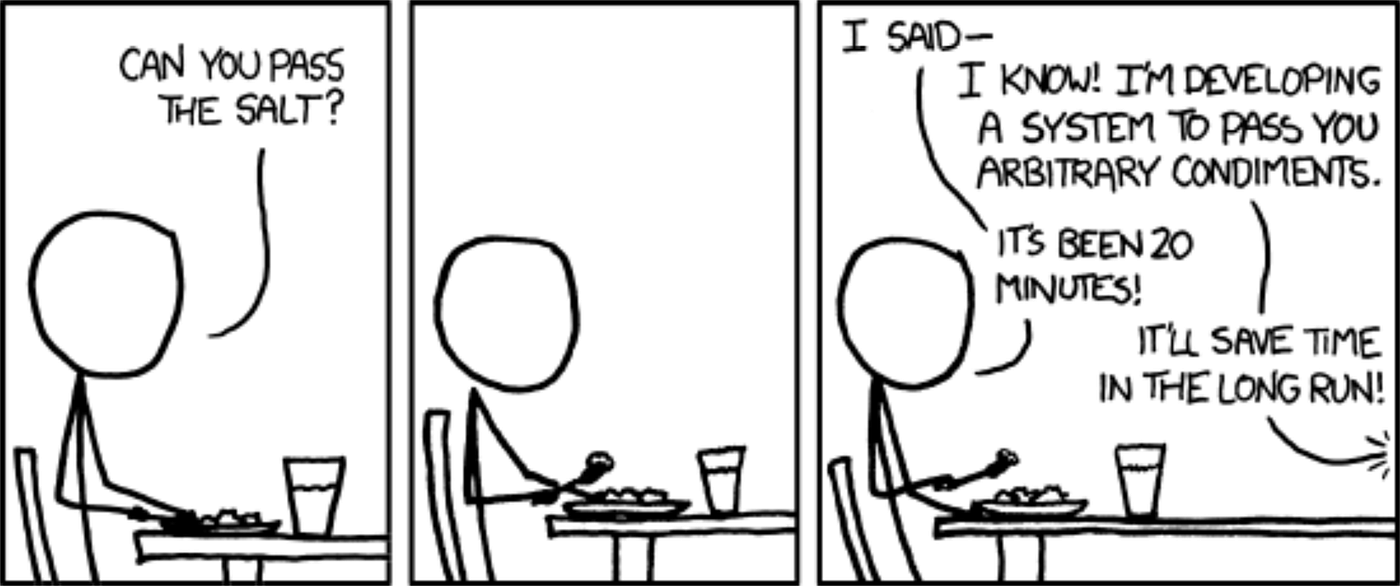
\includegraphics[height=0.25\textheight]{YAGNI}
            \end{center}
        \end{onlyenv}
        \begin{varblock}{quote}[\textwidth]{Experience makes you better}[A comment on Reddit]<only@2->
            \footnotesize
            Here's the truth with these patterns/paradigms.
            A junior dev will ignore them and code something simple that will not scale.
            A mid level will understand abstraction but over engineer a lot of things because they lack the experience to judge whether they are appropriate in the context of their work.
            Seniors will go back to simple things and postpone until it's really needed to make it more complex, because life taught them the costs of premature optimizations.
            The final level is when you understand that all of these are concepts that are good to know but none is a universal truth.
            [...]
        \end{varblock}
        \vspace{-1mm}
        \begin{onlyenv}<3->
            \begin{varblock}{example}[\textwidth]{I need to check whether a vector contains an element:}<only@3>
                \begin{lstlisting}[style=MyCpp]
                    // A (too?) specific implementation
                    bool isElementInVector(const std::vector<double>& data,
                                           double value)
                    {
                        auto it = std::find(data.begin(), data.end(), value);
                        return it != data.end();
                    }
                \end{lstlisting}
            \end{varblock}
            \begin{varblock}{example}[\textwidth]{I need to check whether a vector contains an element:}<only@4>
                \begin{lstlisting}[style=MyCpp]
                    template<typename T>
                    bool isElementInVector(const std::vector<T>& data,
                                           const T& value)
                    {
                        auto it = std::find(data.begin(), data.end(), value);
                        return it != data.end();
                    }
                \end{lstlisting}
            \end{varblock}
            \begin{varblock}{example}[\textwidth]{I need to check whether a vector contains an element:}<only@5>
                \begin{lstlisting}[style=MyCpp]
                    // Probably NOT straight away!
                    template<typename Container, typename Item>
                    bool contains(const Container& container, const Item& value)
                    {
                        // Some implementation possibly calling container
                        // member find or ::std::find if container has none
                    }
                \end{lstlisting}
            \end{varblock}
        \end{onlyenv}
    \end{overlayarea}
    \FrameRemark<1>{Ron Jeffries is a co-founder of extreme programming (XP) philosophy.}
\end{frame}
%~~~~~~~~~~~~~~~~~~~~~~~~~~~~~~~~~~~~~~~~~~~~%
\subsection{Optimisation}
%~~~~~~~~~~~~~~~~~~~~~~~~~~~~~~~~~~~~~~~~~~~~%
\begin{frame}{Do not be disappointed}{I have only a couple of slides about optimisation}
    \begin{varblock}{quote}[0.8\textwidth]{}
        \normalfont\Large\PS{\textbf{Correctness}} comes before \alert{performance}!
    \end{varblock}
    \begin{varblock*}{}[0.72\textwidth]{Steps needed seeking for speed:}
        \begin{enumerate}
            \item Write \textbf{enough} tests
            \item Profile the code
            \item Benchmark the part you want optimise
            \item Change the code \uncover<2>{{\small$\;\leftarrow\;$ \alert{\textbf{Optimisation is not just this!}}}}
            \item Make sure tests still pass
            \item \CPP|goto| \;\MakeEnumerateBox{3} or \MakeEnumerateBox{2}
        \end{enumerate}
    \end{varblock*}
\end{frame}
%~~~~~~~~~~~~~~~~~~~~~~~~~~~~~~~~~~~~~~~~~~~~%
\begin{frame}{Beware of optimisations}
    \vspace{-5mm}
    \begin{quoteblock}{Premature optimisation}[D. Knuth]
        Programmers waste enormous amounts of time thinking about, or worrying about,
        the speed of noncritical parts of their programs, and these attempts at efficiency
        actually have a strong negative impact when debugging and maintenance are considered.
        We should forget about small efficiencies, say about 97\% of the time:
        \par\smallskip
        \centerline{\alert{\textbf{Premature optimisation is the root of all evil}.}}
        \par\smallskip
        Yet we should not pass up our opportunities in that critical 3\%.
    \end{quoteblock}
    \vspace{-3mm}
    \begin{itemize}
        \item Compiler do more and more a better job!
        \item Use optimisations flags (e.g. \PP{\texttt{-O1}}, \PP{\texttt{-O3}} with \texttt{g++} and \texttt{clang})
        \item \alert{Never} sacrifice clean code in name of \textbf{claimed} better performance!
        \item Only optimise after having used a profiler and having written tests!
    \end{itemize}
\end{frame}
%~~~~~~~~~~~~~~~~~~~~~~~~~~~~~~~~~~~~~~~~~~~~%
\subsection{Boy scout philosophy}
%~~~~~~~~~~~~~~~~~~~~~~~~~~~~~~~~~~~~~~~~~~~~%
\begin{frame}{The boy scout rule}
    \vspace{0mm}
    \begin{columns}[c]
        \hfill
        \begin{column}{0.46\textwidth}
            \vspace{-\medskipamount}
            \begin{varblock}{}[\columnwidth]{}
                \color{PB}Leave the campground cleaner than you found it
            \end{varblock}
            \vspace{-1mm}
            \begin{varblock}{example}[\columnwidth]{}
                \color{PS}Always check in the code cleaner than you checked it out
            \end{varblock}
        \end{column}
        \begin{column}{0.45\textwidth}
            
\includegraphics[width=0.9\textwidth]{Firecamp.jpg}
        \end{column}
    \end{columns}
    \vspace{3mm}
    \begin{itemize}
        \item To clean an existing code base takes time and requires effort
        \item Aim for tiny but continuous progress
        \item Applying the boy scout rule is a way to pay back technical debt
        \item Any IDE will help you in quickly achieving easy refactoring
    \end{itemize}
    \begin{tikzpicture}[remember picture, overlay]
        \path[to] ($(current page.north west)!0.52!(current page.west)+(9mm,0)$) edge[out=180, in=180] ++(0,-18.5mm);
    \end{tikzpicture}
\end{frame}
%===================================================================================================%
    \session{exercise}{Refactor!}
    %-------------------------------%
%  Author: Alessandro Sciarra   %
%    Date: 02 Jul 2025          %
%-------------------------------%

%~~~~~~~~~~~~~~~~~~~~~~~~~~~~~~~~~~~~~~~~~~~~%
\begin{frame}{\alt<1>{A word about refactoring}{Your task}}
    \vspace{-3mm}
    \begin{varblock}{quote}[\textwidth]{A definition}[Wikipedia]
        In computer programming and software design, code refactoring is the process of restructuring existing source code without changing its external behaviour.
        Refactoring is intended to improve the design, structure, and/or implementation of the software, while preserving its functionality.
    \end{varblock}
    \vspace{1mm}
    \begin{overlayarea}{\textwidth}{0.45\textheight}
        \begin{onlyenv}<1>
            \begin{center}
                
\includegraphics[height=0.4\textheight]{Refactoring-I}
                \qquad
                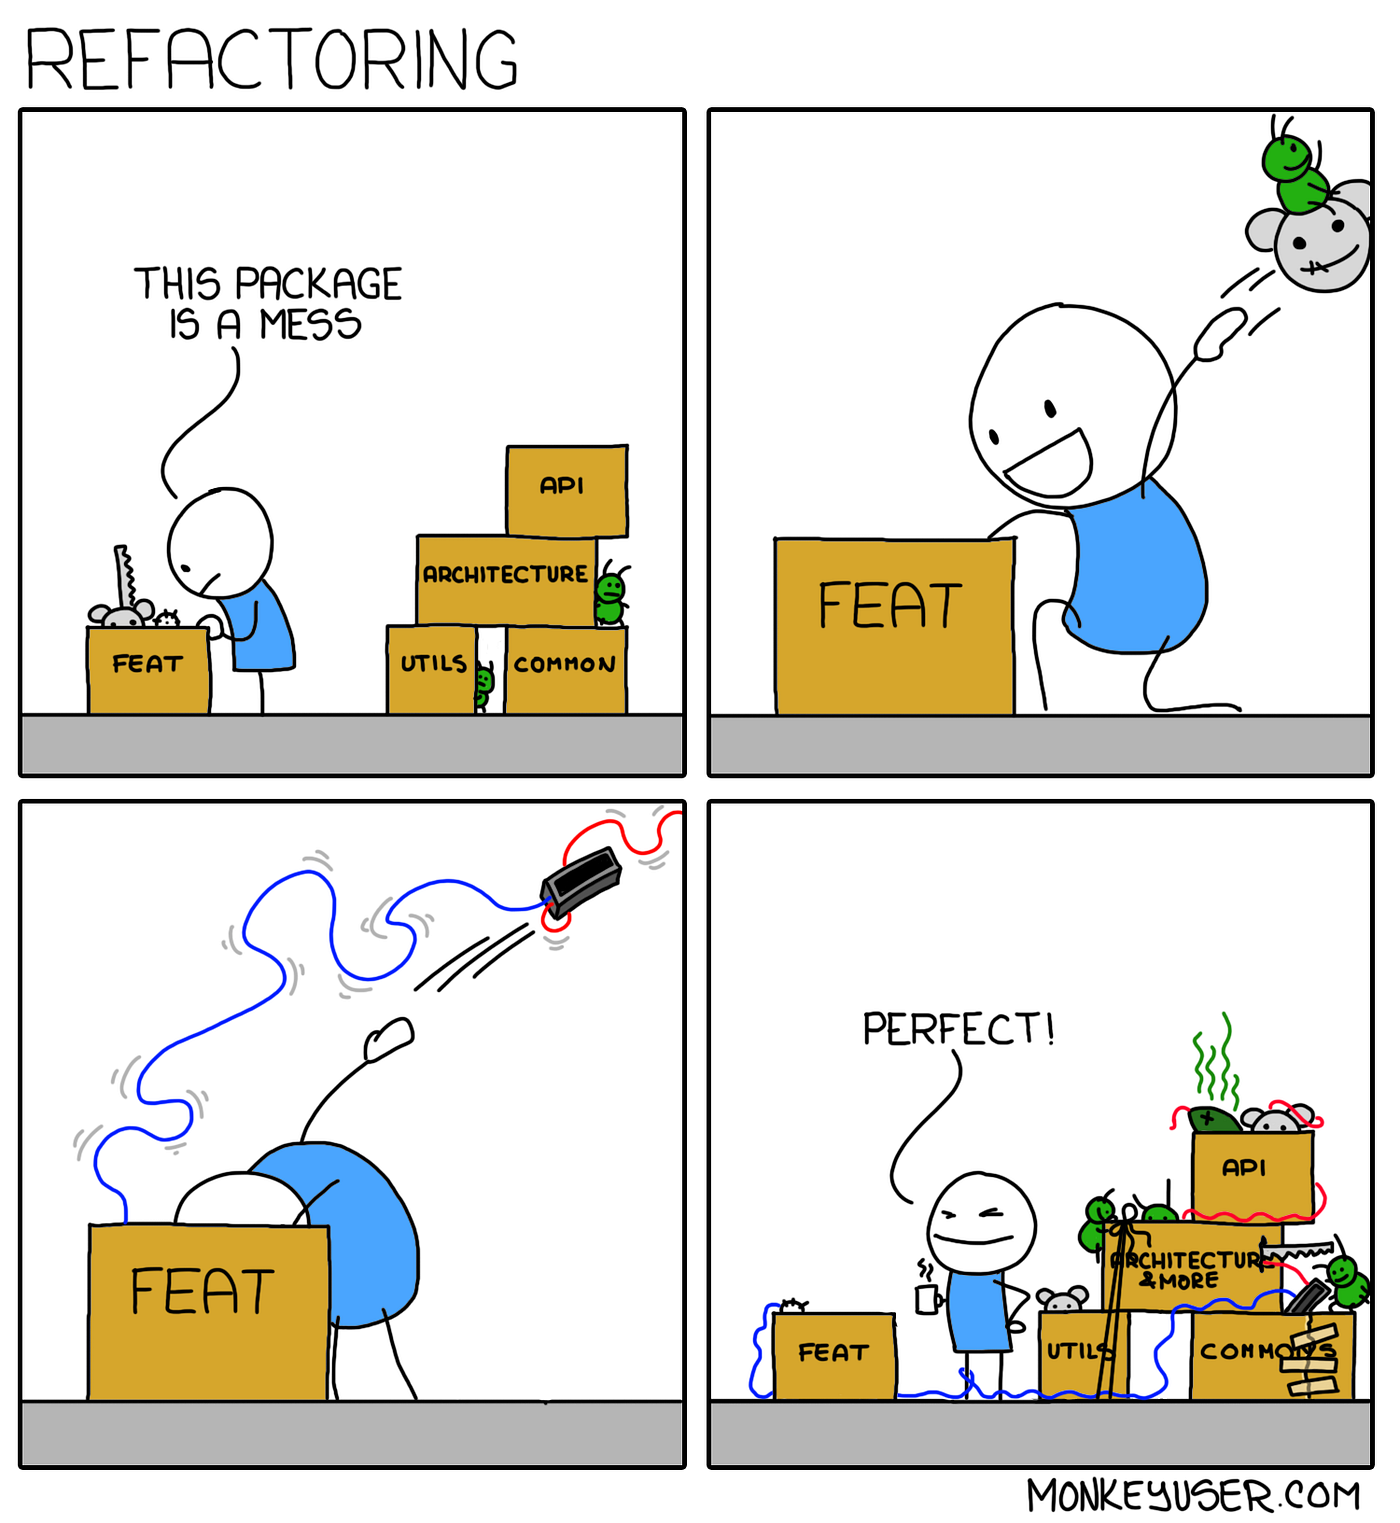
\includegraphics[height=0.4\textheight]{Refactoring-II}
            \end{center}
        \end{onlyenv}
        \begin{onlyenv}<2>
            \begin{enumerate}
                \item Watch out for violations of the learned principles\\
                      \then Any code duplication?\\
                      \then Any part hard to understand?\\
                      \then Any unnecessary generalisation?\\
                \item Improve the code, adding tests first if needed
                \item \alert{Stage, commit and push your work!}
            \end{enumerate}
        \end{onlyenv}
    \end{overlayarea}
\end{frame}
%~~~~~~~~~~~~~~~~~~~~~~~~~~~~~~~~~~~~~~~~~~~~%

    \session{closing}{Sum up and closing}
    %-------------------------------%
%  Author: Alessandro Sciarra   %
%    Date: 26 Jun 2025          %
%-------------------------------%

%~~~~~~~~~~~~~~~~~~~~~~~~~~~~~~~~~~~~~~~~~~~~%
\begin{frame}{Time to reflect on the day}
    \begin{onlyenv}<1>
        \begin{varblock*}{example}[0.7\textwidth]{You have an opportunity after dinner!}
            \begin{itemize}
                \item[\yes] Finish working on exercises in the room
                \item[\yes] Ask further and/or broader questions
                \item[\yes] Enjoy others' discussion
            \end{itemize}
        \end{varblock*}
        \begin{center}
            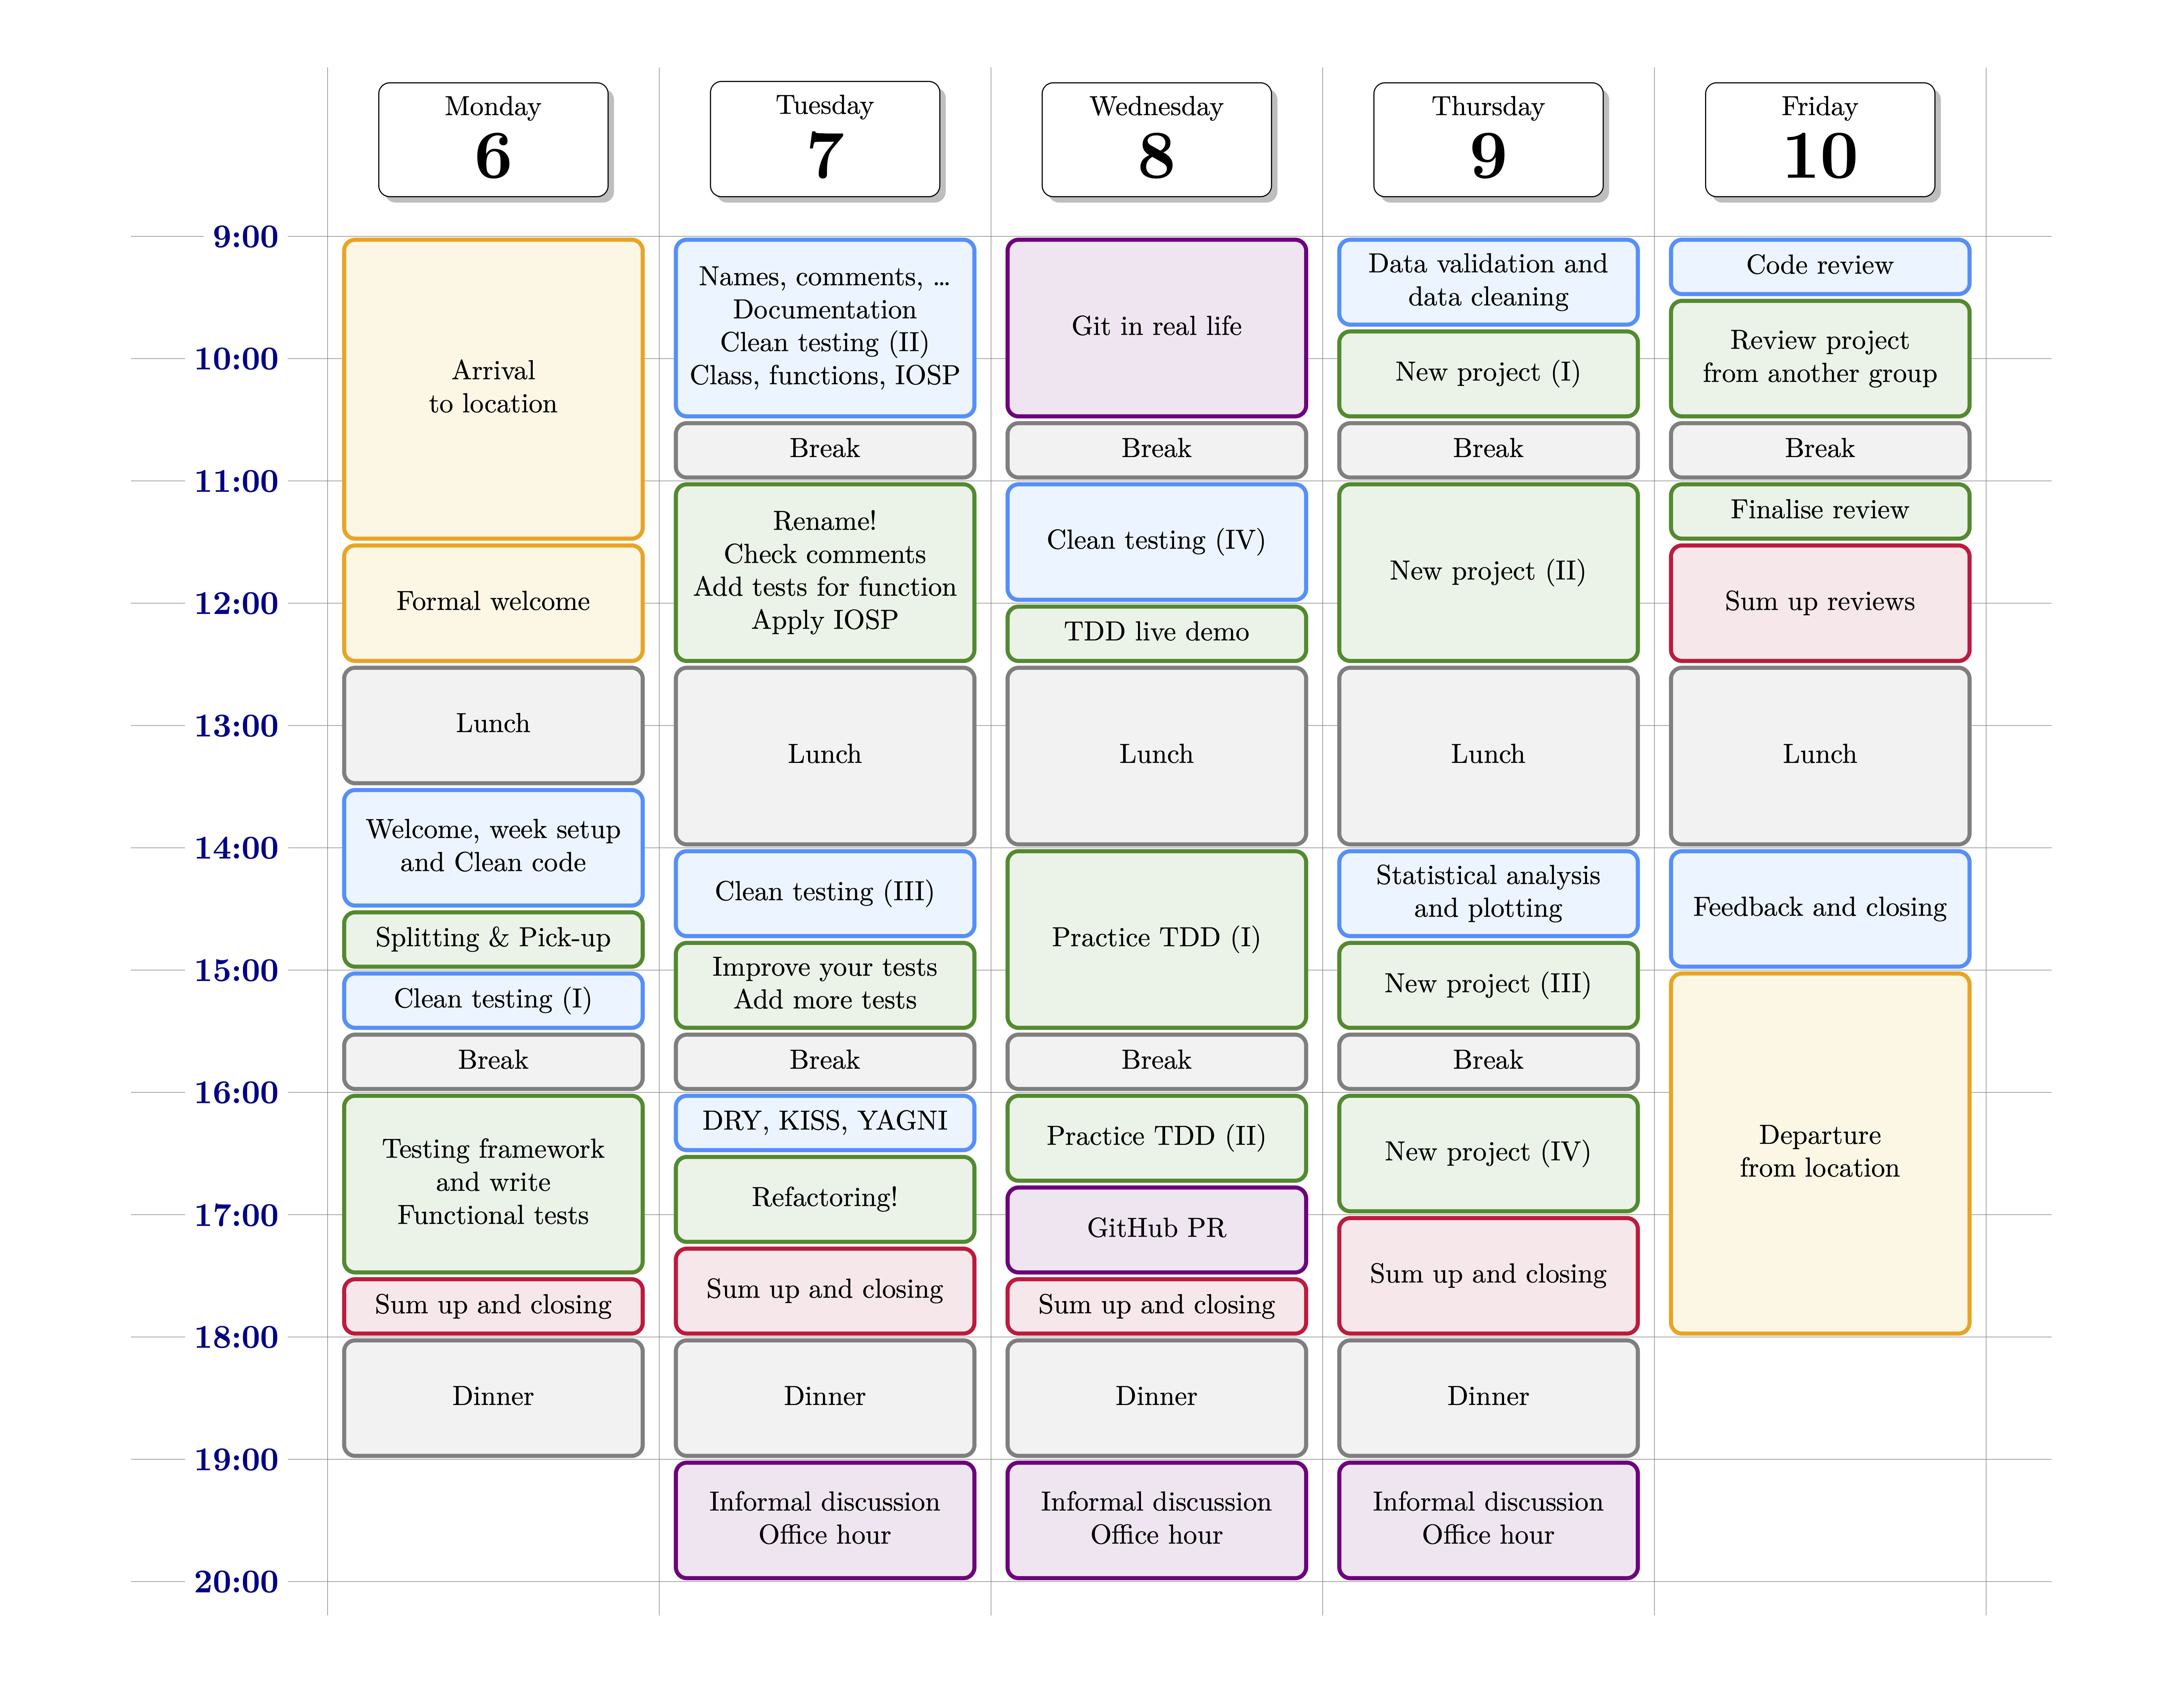
\includegraphics[width=0.6\textwidth, clip, trim=460mm 0mm 400mm 1400mm]{Timetable}\\[1mm]
            It is not mandatory, but you can use it as you wish.
        \end{center}
    \end{onlyenv}
    \begin{onlyenv}<2>
        \begin{enumerate}
            \item Take few minutes to look back at the work done:
                  \begin{itemize}
                      \item How was the code you received?
                      \item What's your general impression?
                      \item Are there unanswered questions?
                      \item Any challenging aspect?
                      \item Are you sceptical? If so, about what?
                  \end{itemize}
            \item Report your group experience/work to the whole class.
        \end{enumerate}
        \begin{center}
            
\includegraphics[width=0.3\textwidth]{Change-chance}
        \end{center}
    \end{onlyenv}
\end{frame}
%~~~~~~~~~~~~~~~~~~~~~~~~~~~~~~~~~~~~~~~~~~~~%

\end{document}
